\section{Dataset Analysis and Experiments}
\subsection{Dataset Preparation and Preprocessing}
\begin{minted}{py}
def split_and_visualize(X, y, dataset_name: str):
    splits = {}

    for ratio in [0.4, 0.6, 0.8, 0.9]:
        X_train, X_test, y_train, y_test = train_test_split(
            X, y, train_size=ratio, stratify=y, shuffle=True, random_state=42
        )

        splits[ratio] = (X_train, X_test, y_train, y_test)

    return splits
\end{minted}
\begin{flushleft}
	To shuffle the dataset and ensure it is split in a stratified fashion, we use the \texttt{train\_test\_split} function from \texttt{sklearn.model\_selection}. The function takes the dataset and the target variable as inputs, along with the desired train-test split ratio.
	\begin{itemize}
		\item The \texttt{shuffle} parameter randomizes the order of the samples before splitting.
		\item The \texttt{stratify} parameter ensures the dataset is split in a stratified fashion.
	\end{itemize}
\end{flushleft}

\subsection{Interpreting Classification Report and Confusion Matrix}
\begin{minted}{py}
def train_evaluate_decision_tree(
    X_train,
    y_train,
    X_test,
    y_test,
    dataset_name: str,
    split_ratio,
):
    # Dynamically set feature and class names
    feature_names = X_train.columns.tolist()
    class_names = [str(cls) for cls in np.unique(y_train)]

    # Train model
    clf = DecisionTreeClassifier(criterion="entropy", random_state=42)
    clf.fit(X_train, y_train)

    # Predictions
    y_pred = clf.predict(X_test)

    # Classification Report (with validation)
    print(f"\nClassification Report ({dataset_name}, {display_ratio(split_ratio)}):")
    print(
        classification_report(
            y_test,
            y_pred,
            target_names=class_names,
            labels=np.unique(y_test),  # Ensure alignment with actual classes
        )
    )

    # Confusion Matrix
    sns.heatmap(
        confusion_matrix(y_test, y_pred),
        annot=True,
        fmt="d",
        xticklabels=class_names,
        yticklabels=class_names,
    )
\end{minted}
\begin{flushleft}
	To generate the classification report and confusion matrix:
	\begin{itemize}
		\item The \texttt{classification\_report} function provides a detailed report of the model's performance, including precision, recall, and F1-score for each class.
		\item The \texttt{confusion\_matrix} function generates a matrix that shows the number of correct and incorrect predictions for each class.
	\end{itemize}
\end{flushleft}

%================ Breast Cancer =================%
\clearpage
\subsection{Breast Cancer Wisconsin Dataset}
\subsubsection*{Dataset Description}
\begin{itemize}
	\item \textbf{Description:} The UCI Breast Cancer Wisconsin (Diagnostic) dataset is used for classifying tumors as malignant or benign based on features derived from its imaging data.
	\item \textbf{Dataset Info:} 569 samples, binary labels (malignant vs.\ benign), 30 numeric features.
	\item \textbf{Preprocessing:} shuffle \& stratified split at 40/60, 60/40, 80/20, 90/10.
\end{itemize}

\begin{figure}[H]
	\centering
	\begin{subfigure}{0.45\textwidth}
		\centering
		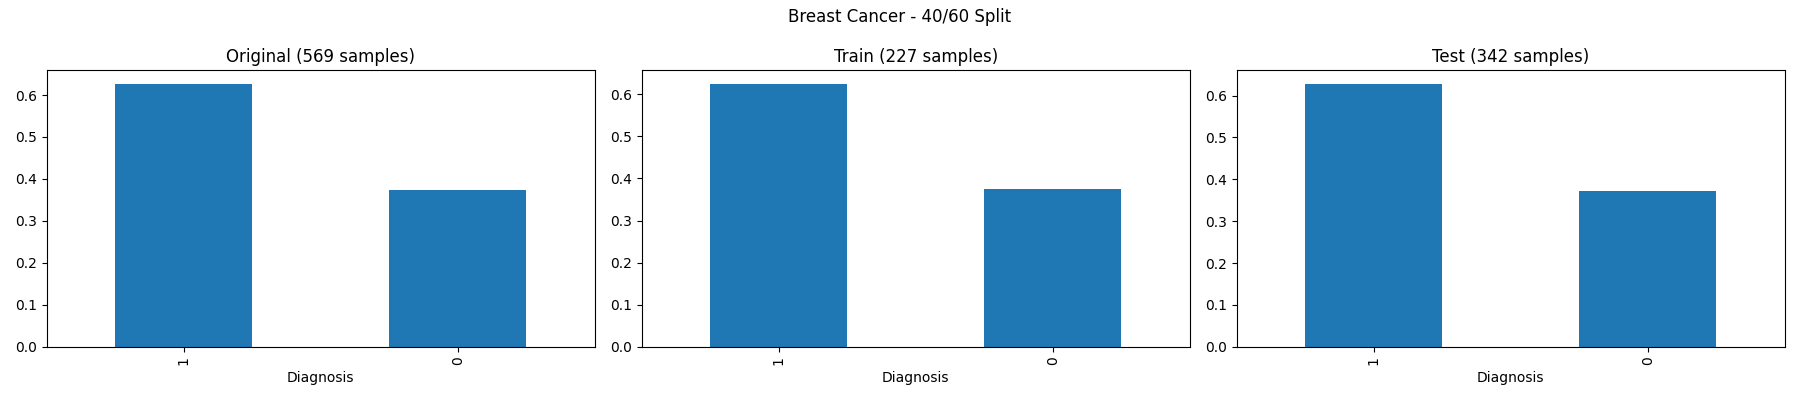
\includegraphics[width=\textwidth]{imgs/class_dist/class_dist__breast_cancer__40_vs_60.png}
		\caption{Breast Cancer: class distribution (40/60 split).}\label{fig:bc-cd-40-60}
	\end{subfigure}
	\hfill
	\begin{subfigure}{0.45\textwidth}
		\centering
		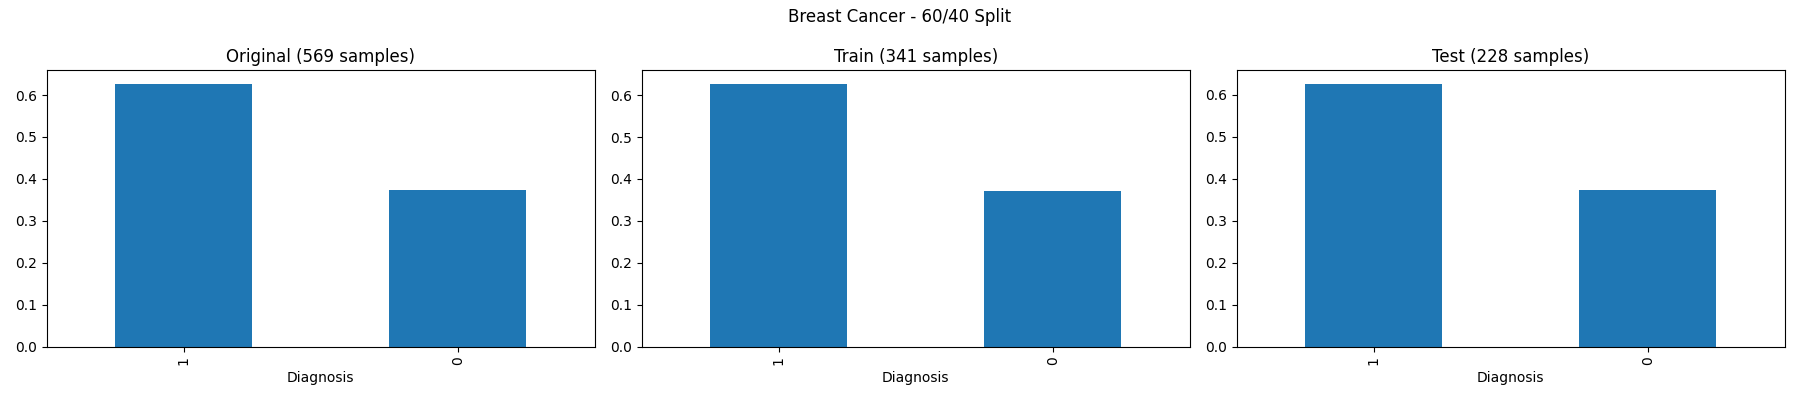
\includegraphics[width=\textwidth]{imgs/class_dist/class_dist__breast_cancer__60_vs_40.png}
		\caption{Breast Cancer: class distribution (60/40 split).}\label{fig:bc-cd-60-40}
	\end{subfigure}
	\hfill
	\begin{subfigure}{0.45\textwidth}
		\centering
		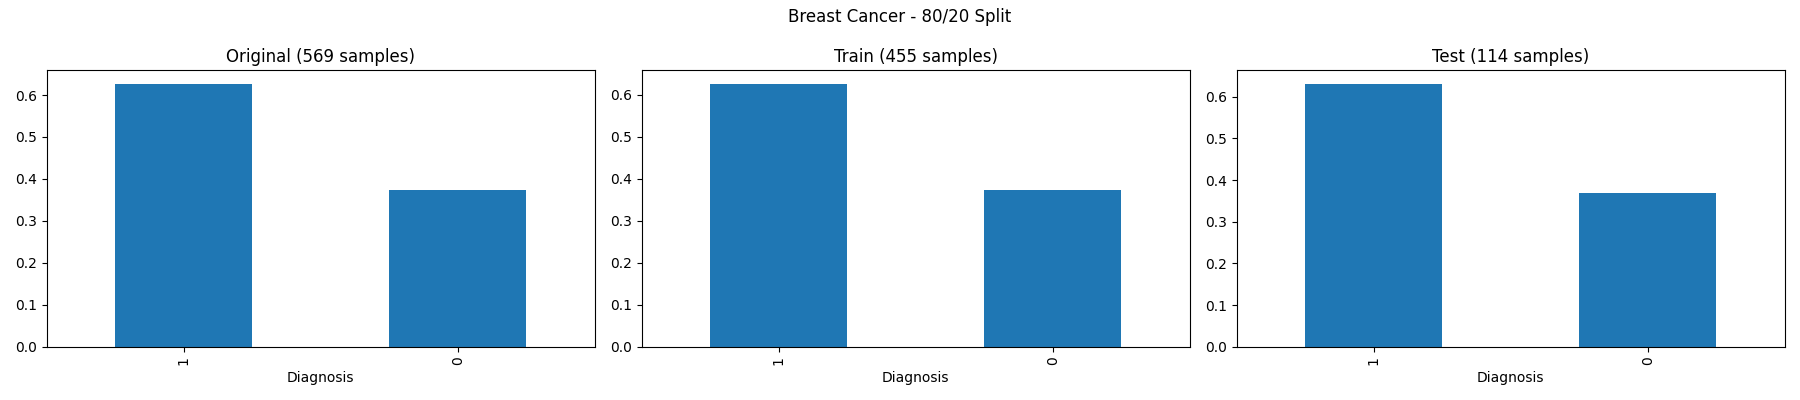
\includegraphics[width=\textwidth]{imgs/class_dist/class_dist__breast_cancer__80_vs_20.png}
		\caption{Breast Cancer: class distribution (80/20 split).}\label{fig:bc-cd-80-20}
	\end{subfigure}
	\hfill
	\begin{subfigure}{0.45\textwidth}
		\centering
		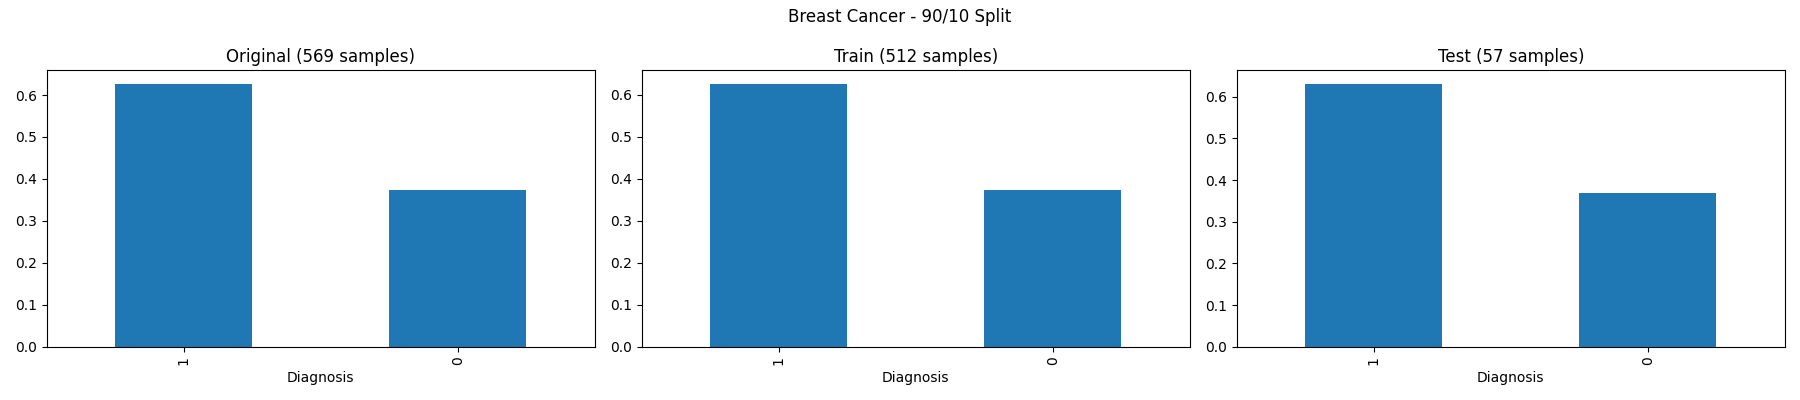
\includegraphics[width=\textwidth]{imgs/class_dist/class_dist__breast_cancer__90_vs_10.png}
		\caption{Breast Cancer: class distribution (90/10 split).}\label{fig:bc-cd-90-10}
	\end{subfigure}

	\caption{Class distributions}\label{fig:bc-cd-all}
\end{figure}

\clearpage
\subsubsection*{Building Decision Tree Classifiers for each train/test proportions}
\begin{figure}[H]
	\centering
	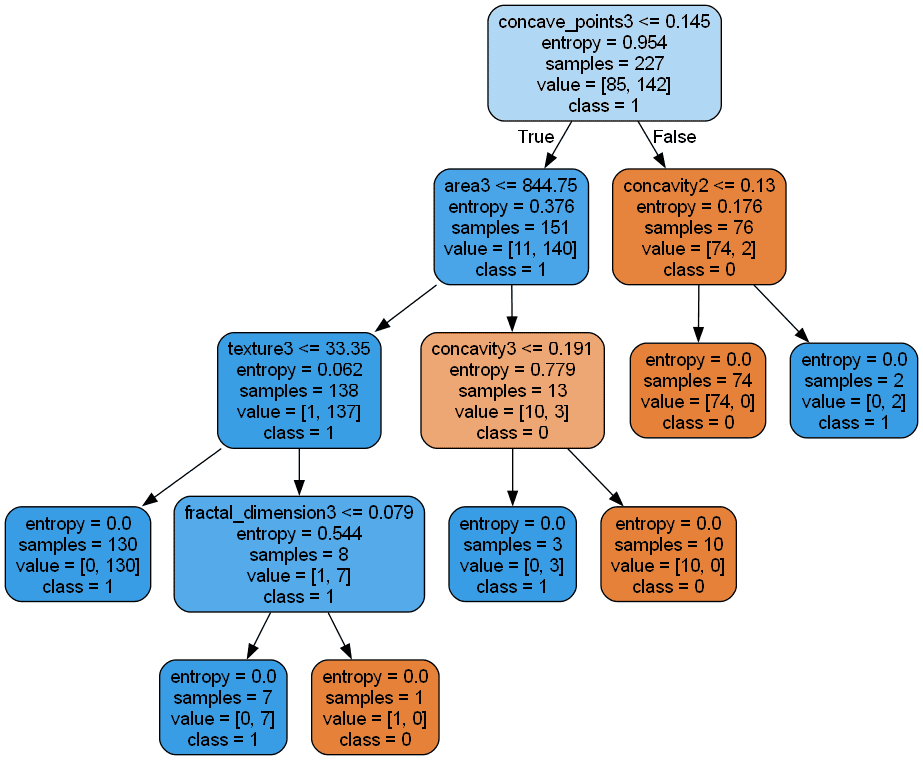
\includegraphics[width=0.65\textwidth]{imgs/dt-mini/dt__breast_cancer__40_vs_60.png}
	\caption{Breast Cancer: decision tree for 40/60 split.}\label{fig:bc-dt-40-60}
\end{figure}
\begin{figure}[H]
	\centering
	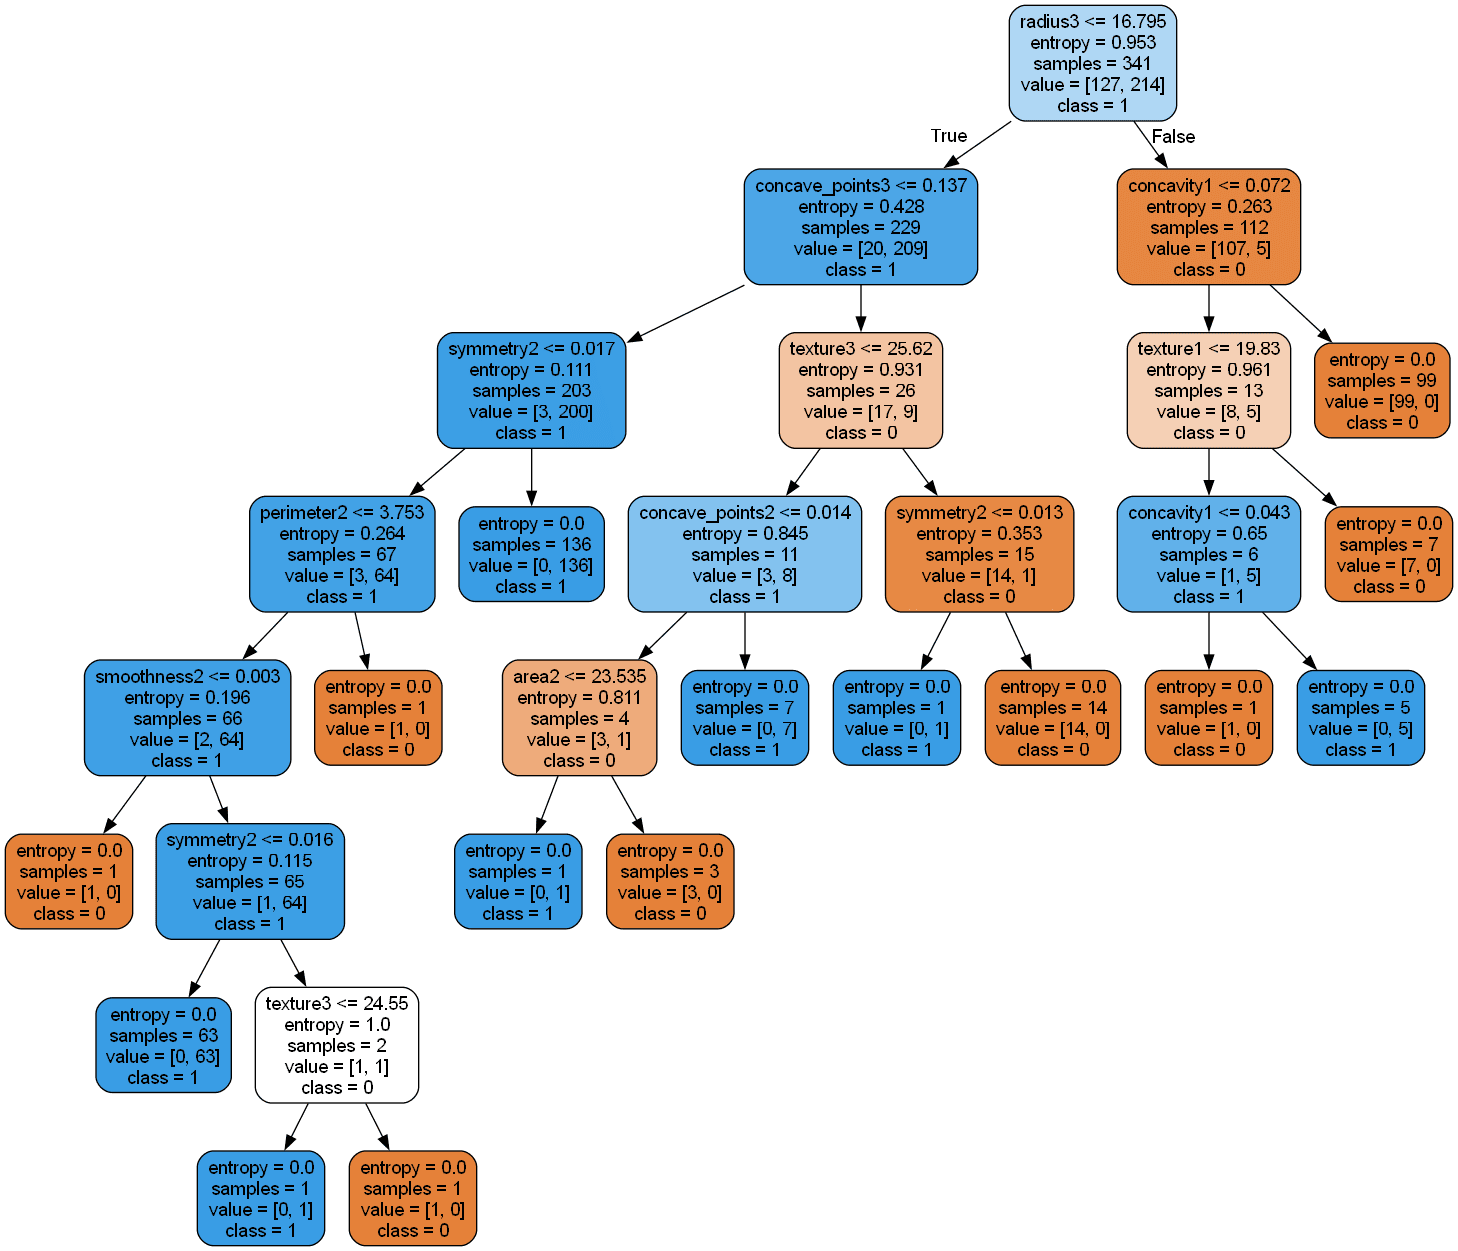
\includegraphics[width=0.65\textwidth]{imgs/dt-mini/dt__breast_cancer__60_vs_40.png}
	\caption{Breast Cancer: decision tree for 60/40 split.}\label{fig:bc-dt-60-40}
\end{figure}
\begin{figure}[H]
	\centering
	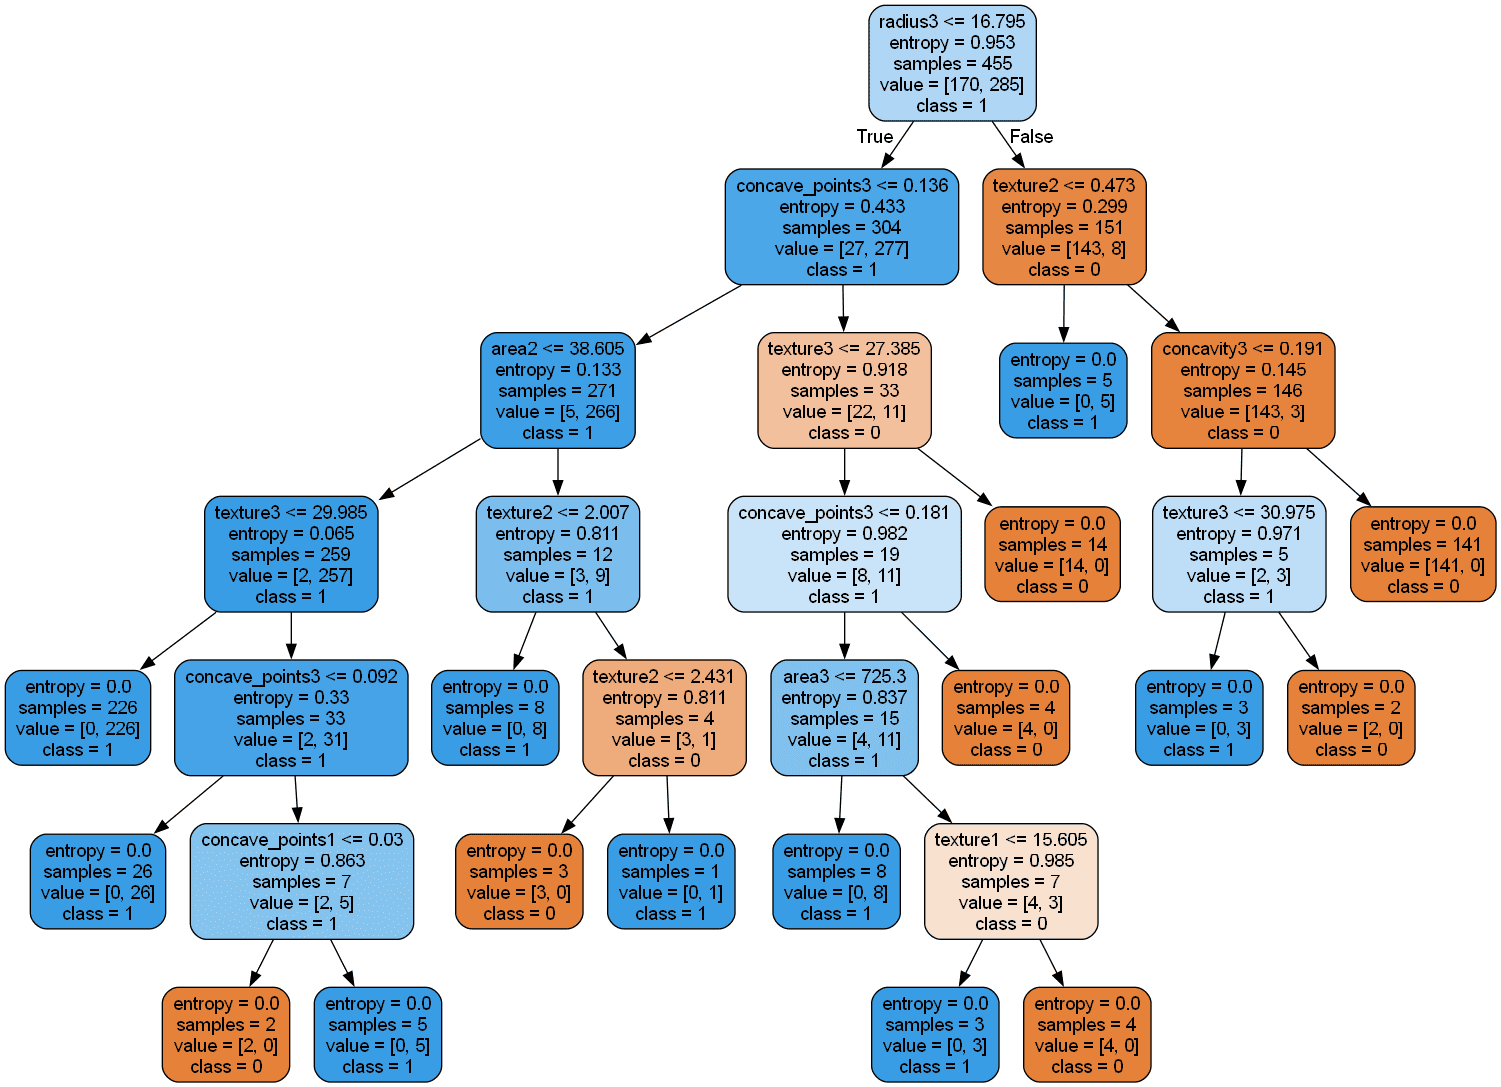
\includegraphics[width=0.65\textwidth]{imgs/dt-mini/dt__breast_cancer__80_vs_20.png}
	\caption{Breast Cancer: decision tree for 80/20 split.}\label{fig:bc-dt-80-20}
\end{figure}
\begin{figure}[H]
	\centering
	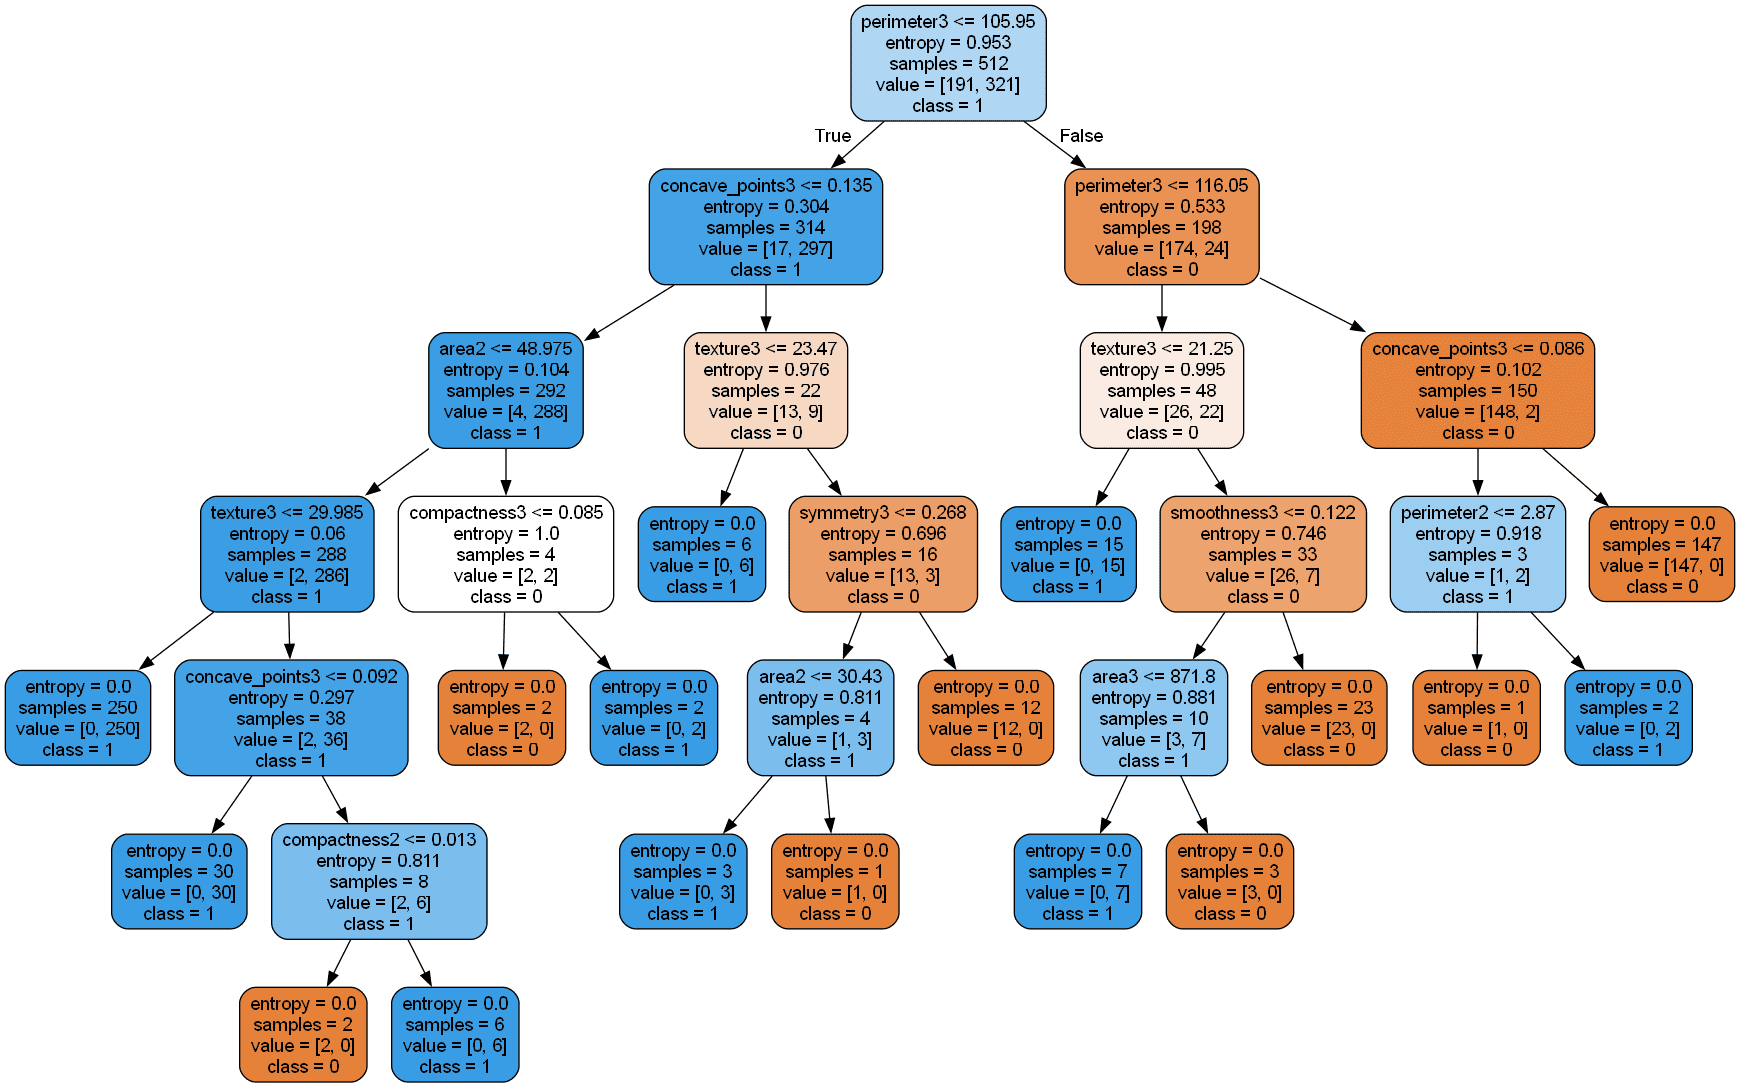
\includegraphics[width=0.65\textwidth]{imgs/dt-mini/dt__breast_cancer__90_vs_10.png}
	\caption{Breast Cancer: decision tree for 90/10 split.}\label{fig:bc-dt-90-10}
\end{figure}

\clearpage
\subsubsection*{Evaluating the decision tree classifiers}
\begin{figure}[H]
	\centering
	\begin{subfigure}{0.45\textwidth}
		\centering
		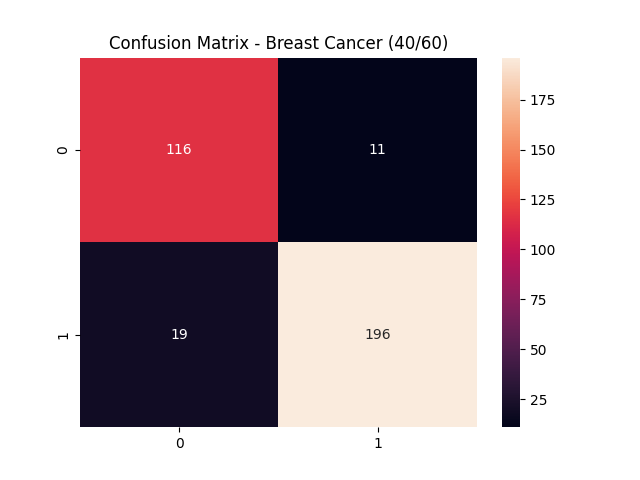
\includegraphics[width=\textwidth]{imgs/confusion_mat/confusion_mat__breast_cancer__40_vs_60.png}
		\caption{Breast Cancer: confusion matrix (40/60 split).}\label{fig:bc-cm-40-60}
	\end{subfigure}
	\hfill
	\begin{subfigure}{0.45\textwidth}
		\centering
		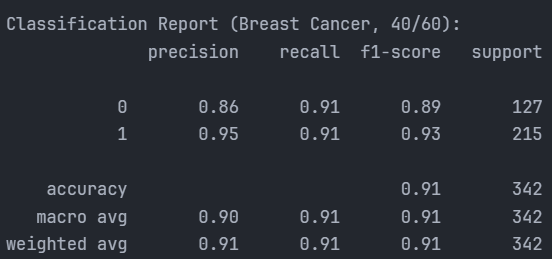
\includegraphics[width=\textwidth]{imgs/confusion_mat/class_rp__breast_cancer__40_vs_60.png}
		\caption{Breast Cancer: Classification Report (40/60 split).}\label{fig:bc-cr-40-60}
	\end{subfigure}

	\caption{Classification Report and Confusion Matrix (40/60 split)}\label{fig:bc-eval-40-60}
\end{figure}
\begin{figure}[H]
	\centering
	\begin{subfigure}{0.45\textwidth}
		\centering
		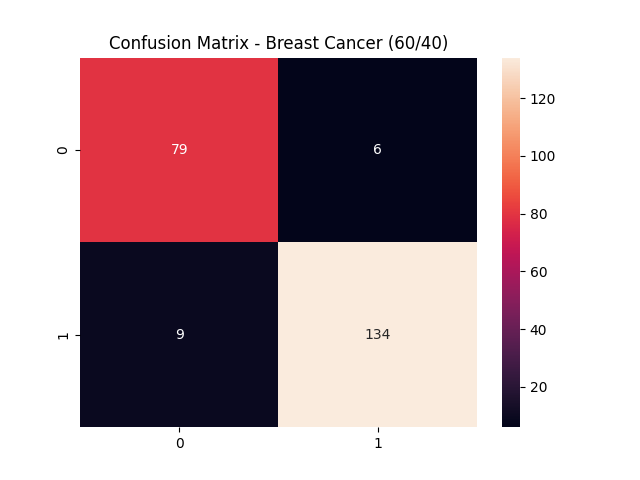
\includegraphics[width=\textwidth]{imgs/confusion_mat/confusion_mat__breast_cancer__60_vs_40.png}
		\caption{Breast Cancer: confusion matrix (60/40 split).}\label{fig:bc-cm-60-40}
	\end{subfigure}
	\hfill
	\begin{subfigure}{0.45\textwidth}
		\centering
		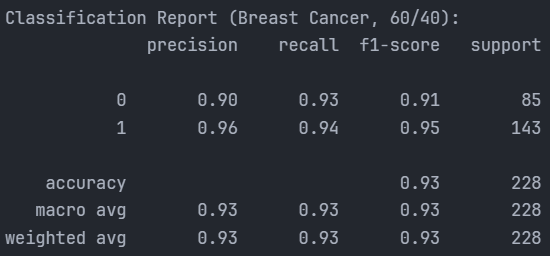
\includegraphics[width=\textwidth]{imgs/confusion_mat/class_rp__breast_cancer__60_vs_40.png}
		\caption{Breast Cancer: Classification Report (60/40 split).}\label{fig:bc-cr-60-40}
	\end{subfigure}

	\caption{Classification Report and Confusion Matrix (60/40 split)}\label{fig:bc-eval-60-40}
\end{figure}
\begin{figure}[H]
	\centering
	\begin{subfigure}{0.45\textwidth}
		\centering
		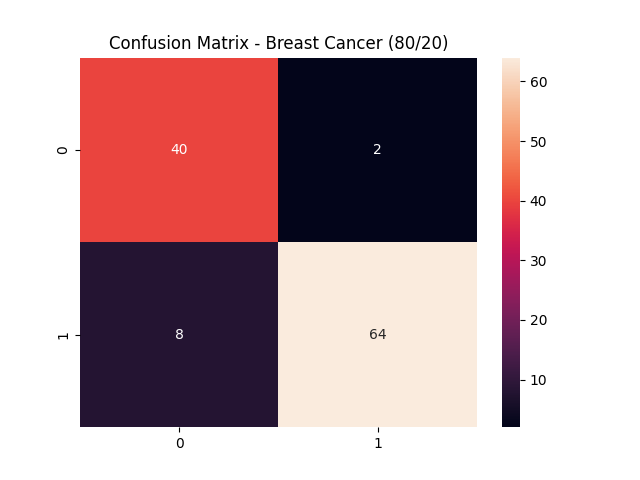
\includegraphics[width=\textwidth]{imgs/confusion_mat/confusion_mat__breast_cancer__80_vs_20.png}
		\caption{Breast Cancer: confusion matrix (80/20 split).}\label{fig:bc-cm-80-20}
	\end{subfigure}
	\hfill
	\begin{subfigure}{0.45\textwidth}
		\centering
		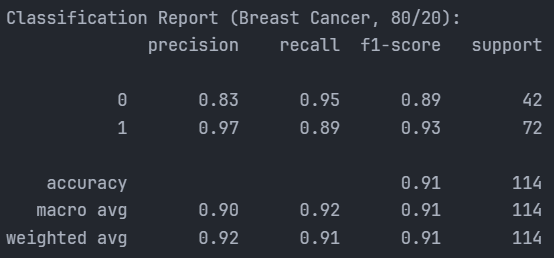
\includegraphics[width=\textwidth]{imgs/confusion_mat/class_rp__breast_cancer__80_vs_20.png}
		\caption{Breast Cancer: Classification Report (80/20 split).}\label{fig:bc-cr-80-20}
	\end{subfigure}

	\caption{Classification Report and Confusion Matrix (80/20 split)}\label{fig:bc-eval-80-20}
\end{figure}
\begin{figure}[H]
	\centering
	\begin{subfigure}{0.45\textwidth}
		\centering
		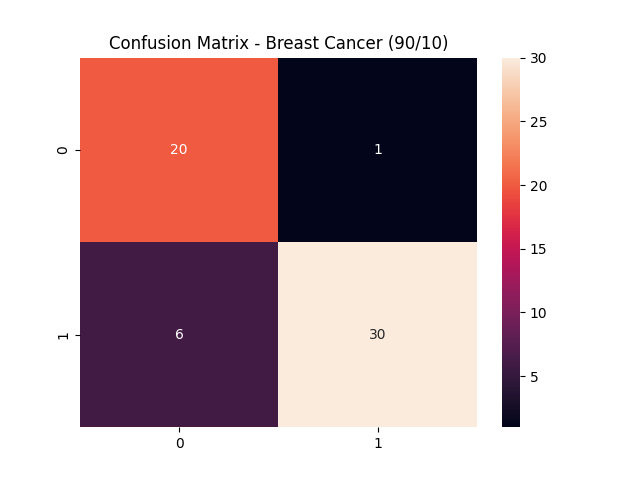
\includegraphics[width=\textwidth]{imgs/confusion_mat/confusion_mat__breast_cancer__90_vs_10.png}
		\caption{Breast Cancer: confusion matrix (90/10 split).}\label{fig:bc-cm-90-10}
	\end{subfigure}
	\hfill
	\begin{subfigure}{0.45\textwidth}
		\centering
		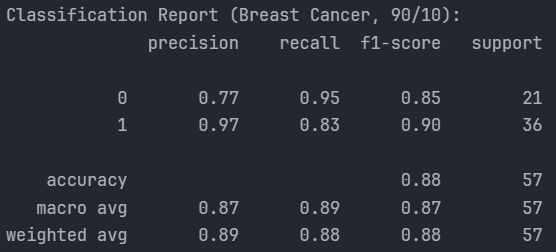
\includegraphics[width=\textwidth]{imgs/confusion_mat/class_rp__breast_cancer__90_vs_10.png}
		\caption{Breast Cancer: Classification Report (90/10 split).}\label{fig:bc-cr-90-10}
	\end{subfigure}

	\caption{Classification Report and Confusion Matrix (90/10 split)}\label{fig:bc-eval-90-10}
\end{figure}
\begin{flushleft}
	Insights into performance of these decision tree classifiers:
	\begin{itemize}
		\item sth
		      \begin{itemize}
			      \item sth
		      \end{itemize}
	\end{itemize}
\end{flushleft}

\clearpage
\subsubsection*{Decision Tree Classifier with Different Depths}
\begin{figure}[H]
	\centering
	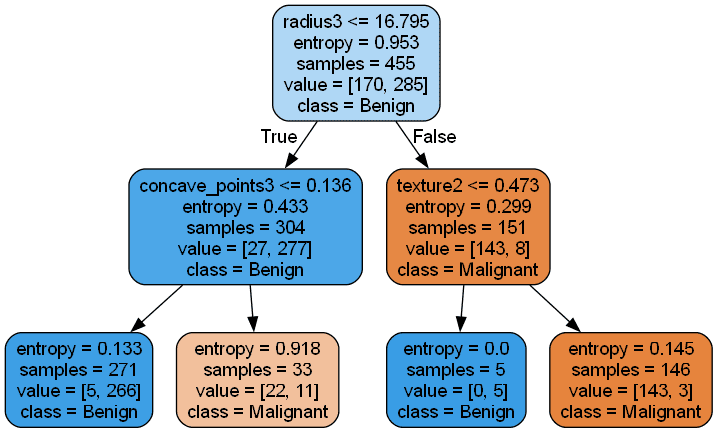
\includegraphics[width=0.65\textwidth]{imgs/dt-mini/dt__breast_cancer__80_vs_20__2.png}
	\caption{Breast Cancer: decision tree with \texttt{max\_depth}=2 (80/20 split).}\label{fig:bc-dt-depth-2}
\end{figure}

\begin{figure}[H]
	\centering
	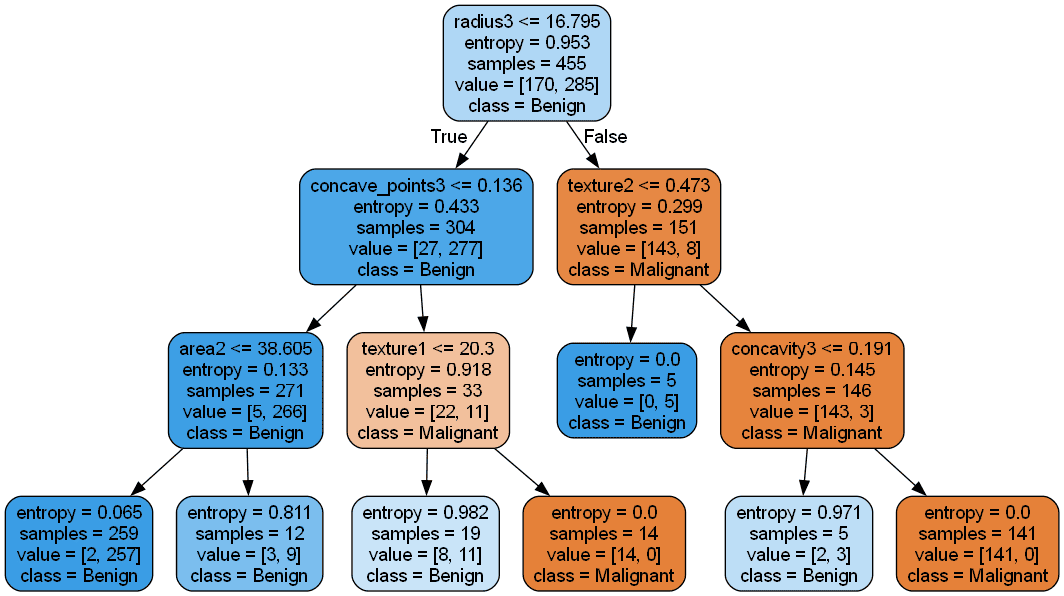
\includegraphics[width=0.65\textwidth]{imgs/dt-mini/dt__breast_cancer__80_vs_20__3.png}
	\caption{Breast Cancer: decision tree with \texttt{max\_depth}=3 (80/20 split).}\label{fig:bc-dt-depth-3}
\end{figure}

\begin{figure}[H]
	\centering
	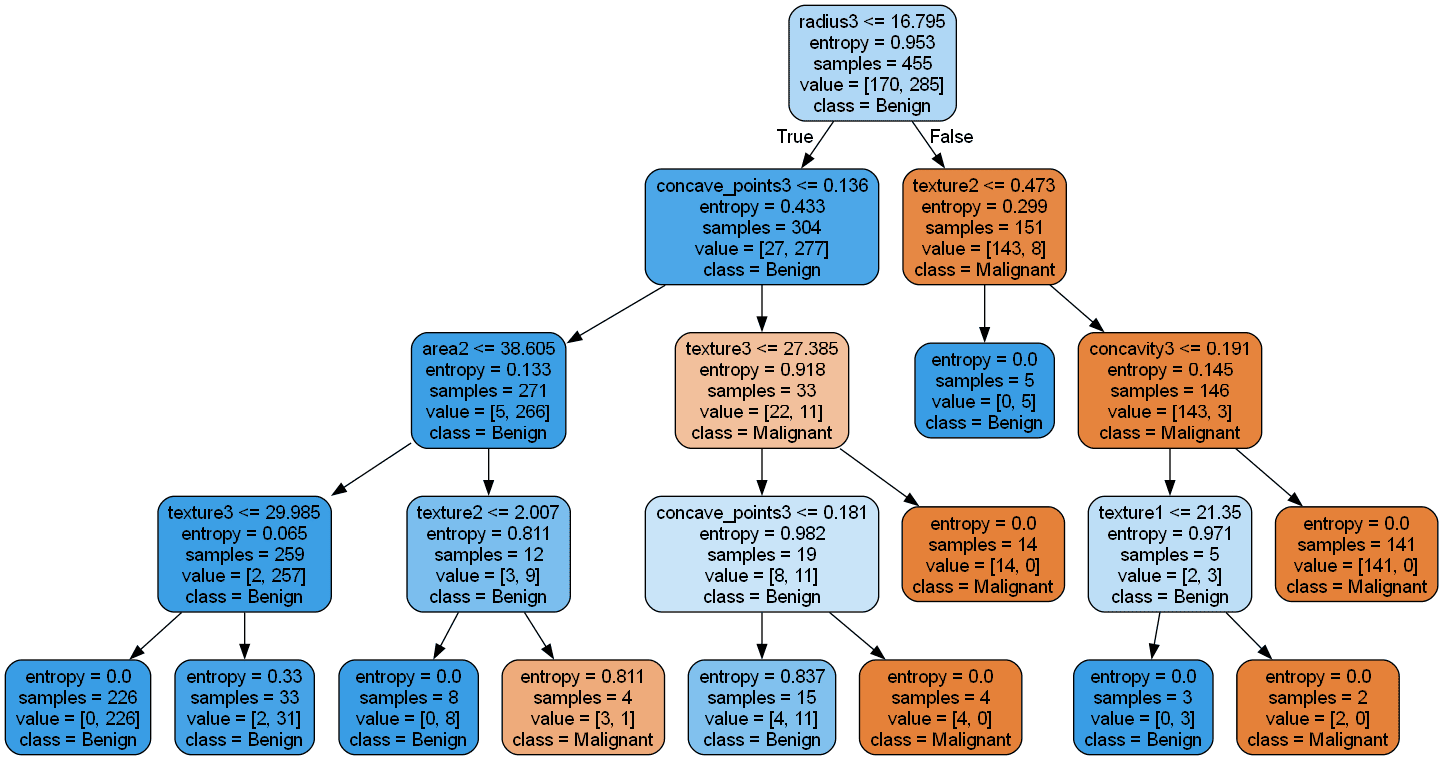
\includegraphics[width=0.65\textwidth]{imgs/dt-mini/dt__breast_cancer__80_vs_20__4.png}
	\caption{Breast Cancer: decision tree with \texttt{max\_depth}=4 (80/20 split).}\label{fig:bc-dt-depth-4}
\end{figure}

\begin{figure}[H]
	\centering
	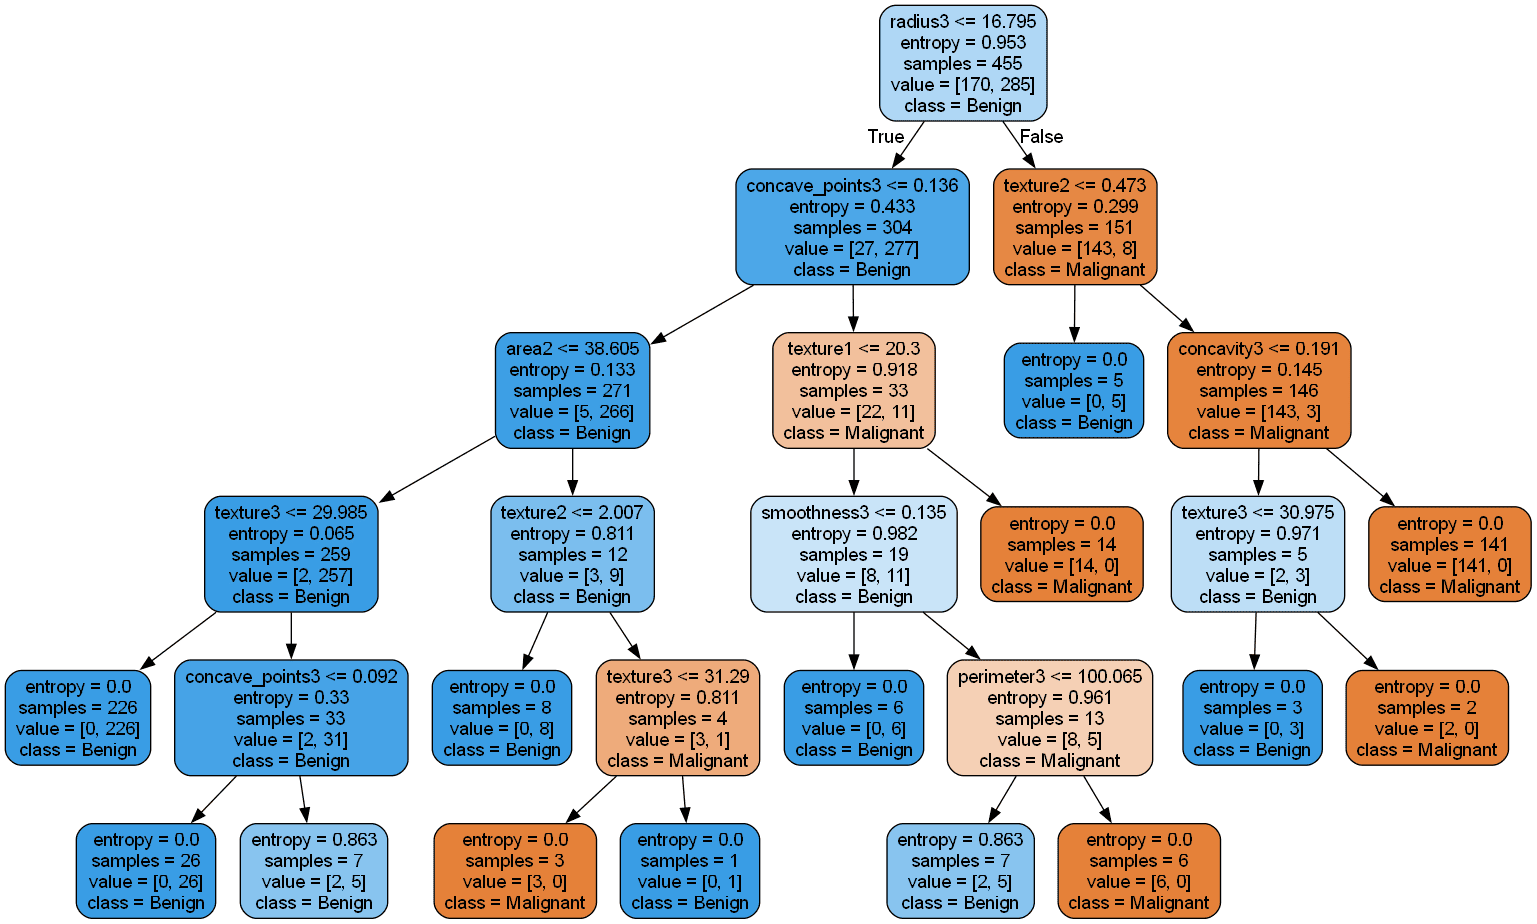
\includegraphics[width=0.65\textwidth]{imgs/dt-mini/dt__breast_cancer__80_vs_20__5.png}
	\caption{Breast Cancer: decision tree with \texttt{max\_depth}=5 (80/20 split).}\label{fig:bc-dt-depth-5}
\end{figure}

\begin{figure}[H]
	\centering
	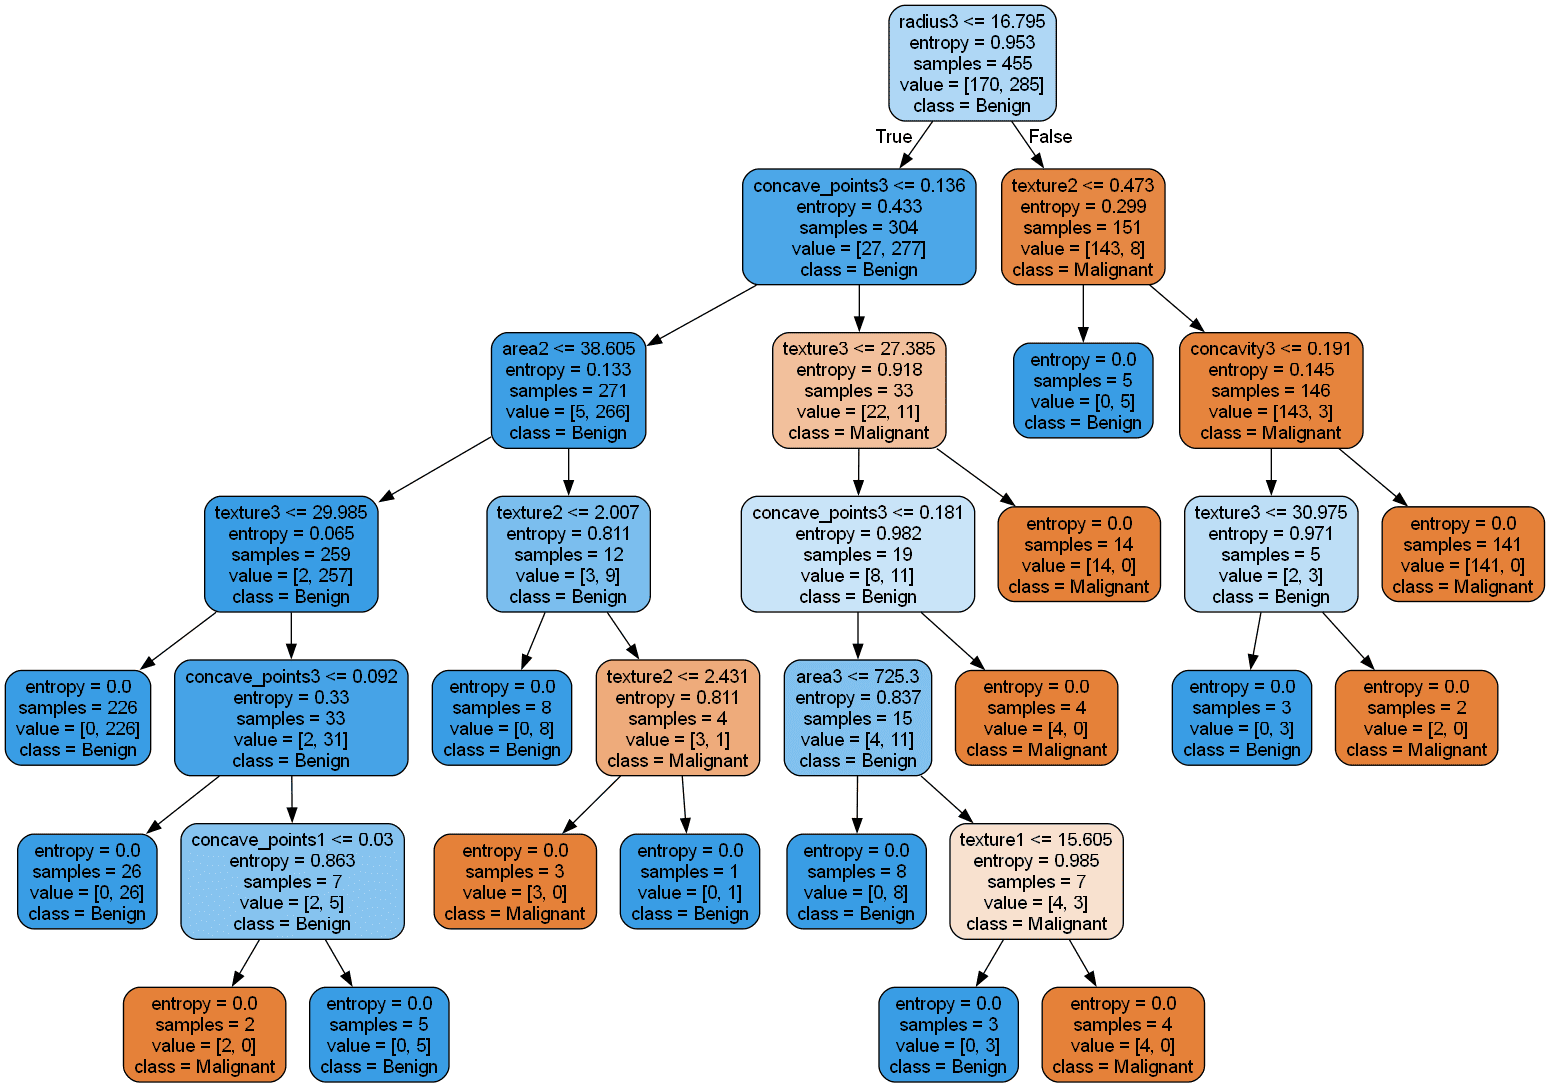
\includegraphics[width=0.65\textwidth]{imgs/dt-mini/dt__breast_cancer__80_vs_20__6.png}
	\caption{Breast Cancer: decision tree with \texttt{max\_depth}=6 (80/20 split).}\label{fig:bc-dt-depth-6}
\end{figure}

\begin{figure}[H]
	\centering
	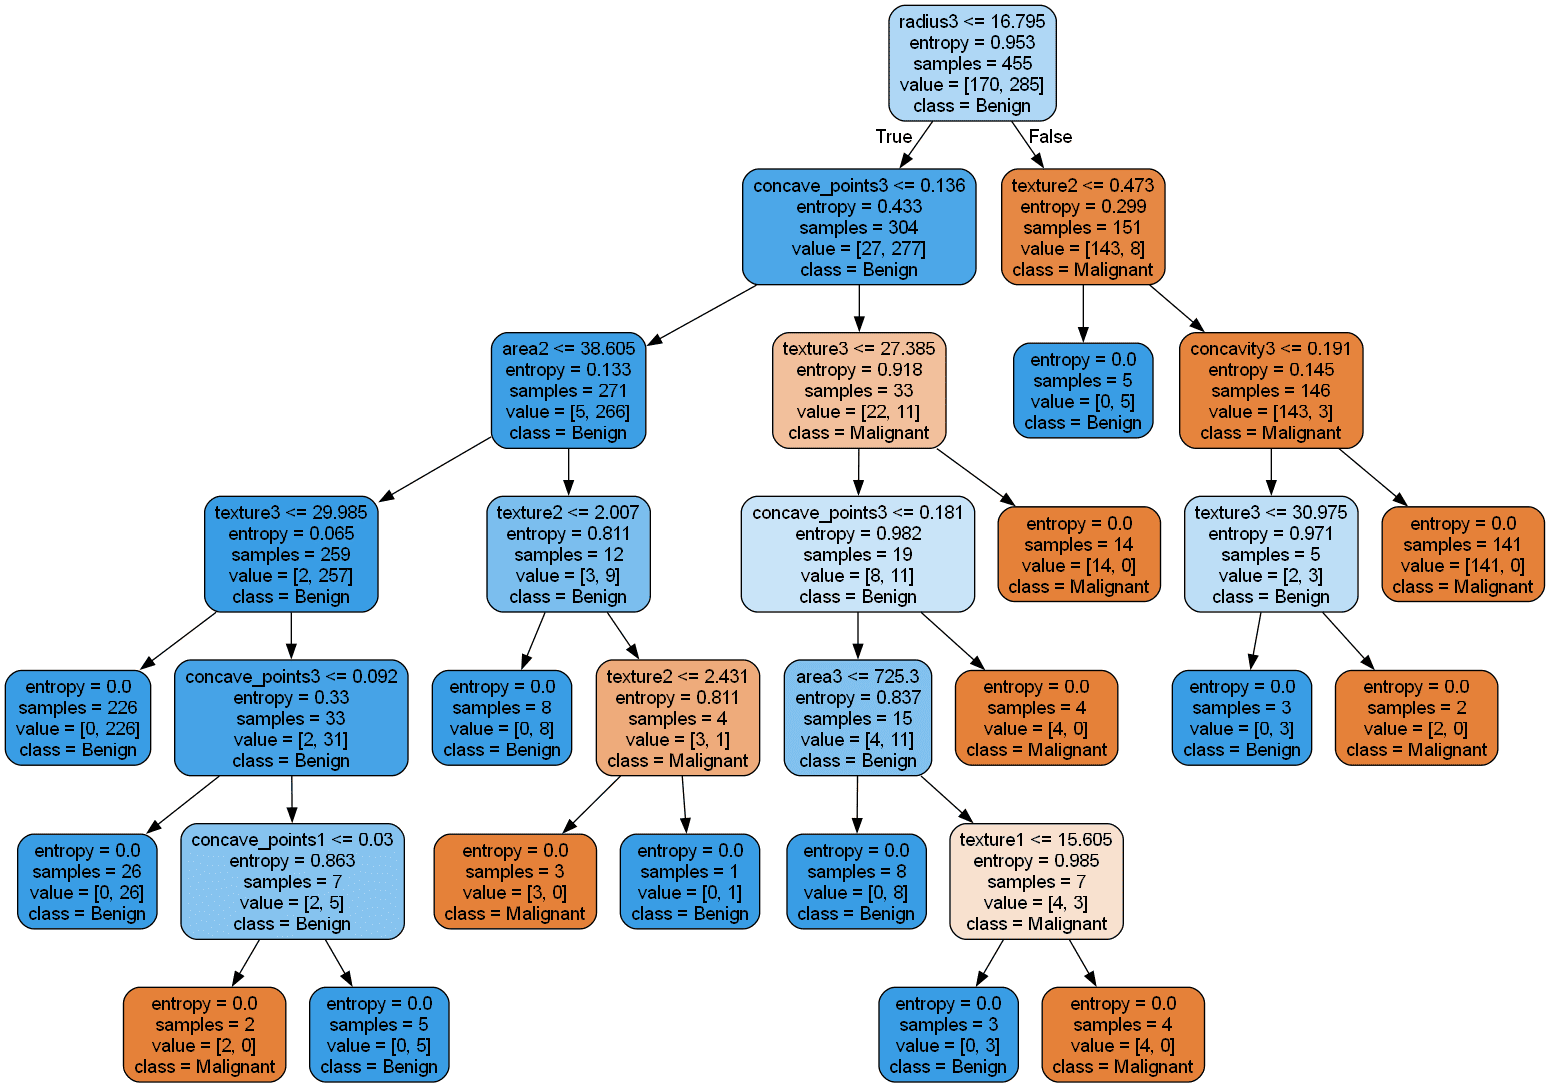
\includegraphics[width=0.65\textwidth]{imgs/dt-mini/dt__breast_cancer__80_vs_20__7.png}
	\caption{Breast Cancer: decision tree with \texttt{max\_depth}=7 (80/20 split).}\label{fig:bc-dt-depth-7}
\end{figure}

\begin{figure}[H]
	\centering
	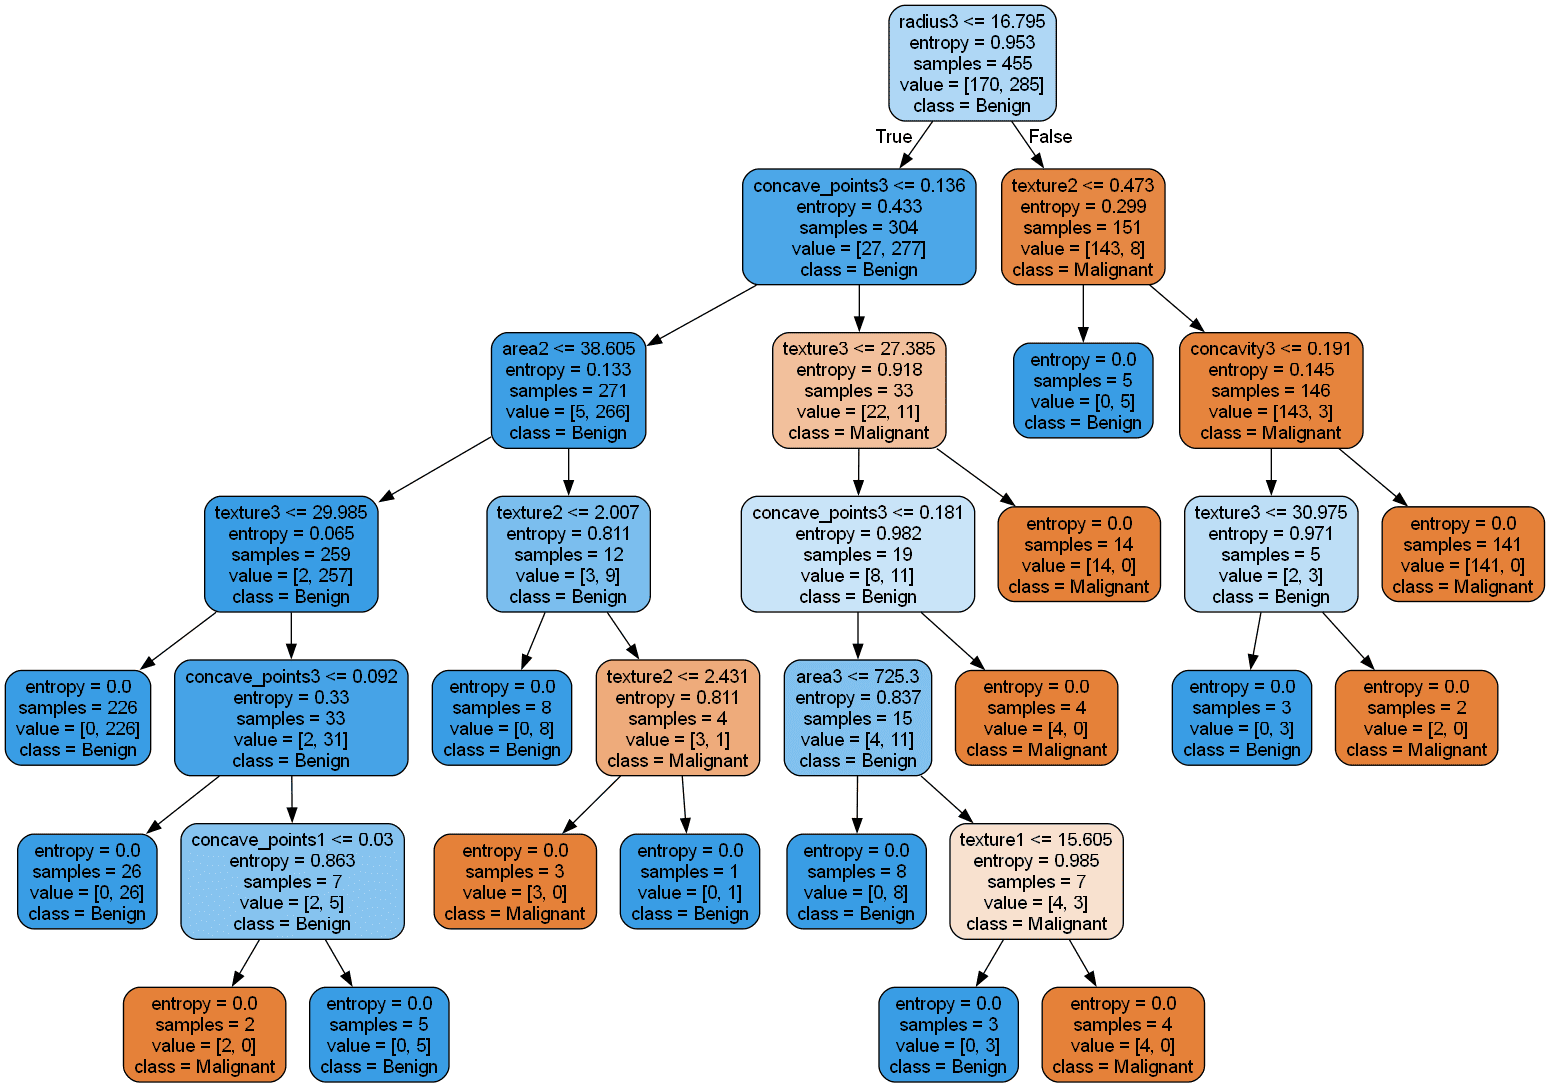
\includegraphics[width=0.65\textwidth]{imgs/dt-mini/dt__breast_cancer__80_vs_20__None.png}
	\caption{Breast Cancer: decision tree with \texttt{max\_depth}=None (80/20 split).}\label{fig:bc-dt-depth-none}
\end{figure}

\begin{figure}[H]
	\centering
	\begin{subfigure}{0.45\textwidth}
		\centering
		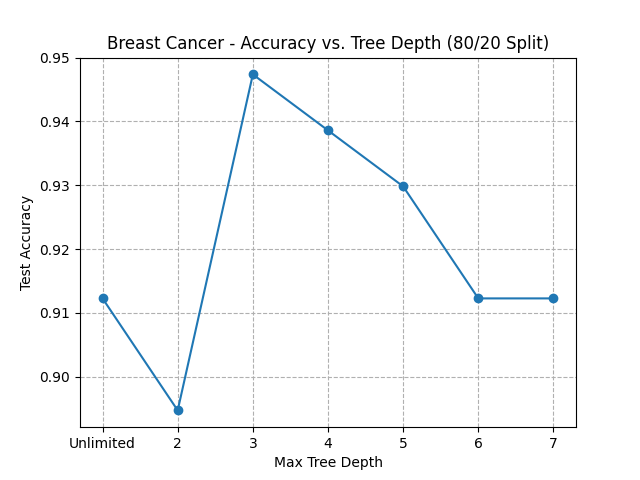
\includegraphics[width=\textwidth]{imgs/accuracy_vs_depth_breast_cancer.png}
	\end{subfigure}
	\hfill
	\begin{subfigure}{0.45\textwidth}
		\centering
		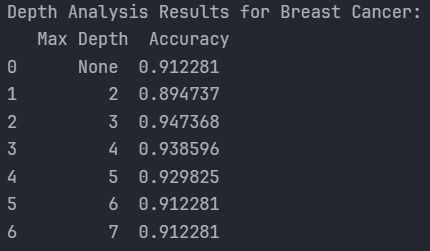
\includegraphics[width=\textwidth]{imgs/accuracy_vs_depth_breast_cancer__analysis.png}
	\end{subfigure}
\end{figure}

\clearpage
\subsubsection*{Insights}
\begin{itemize}
	\item sth
	      \begin{itemize}
		      \item sth
	      \end{itemize}
\end{itemize}

%================ Wine Quality =================%
\clearpage
\subsection{Wine Quality Dataset}
\begin{itemize}
	\item \textbf{Description:} 4,898 samples; original scores 0–10 grouped into Low (0–4), Standard (5–6), High (7–10).
	\item \textbf{Preprocessing:} label encoding, stratified splits at 40/60, 60/40, 80/20, 90/10.
\end{itemize}

\begin{figure}[H]
	\centering
	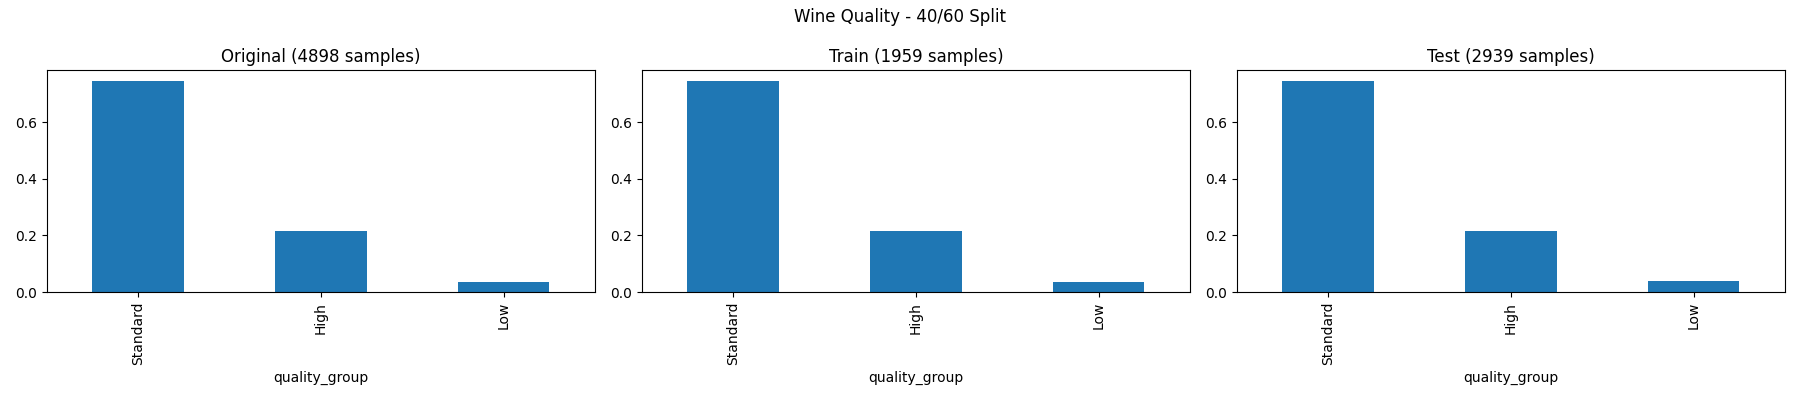
\includegraphics[width=0.6\textwidth]{imgs/class_dist/class_dist__wine_quality__40_vs_60.png}
	\caption{Wine Quality: class distribution (40/60 split).}\label{fig:wq-cd-40-60}
\end{figure}

\begin{figure}[H]
	\centering
	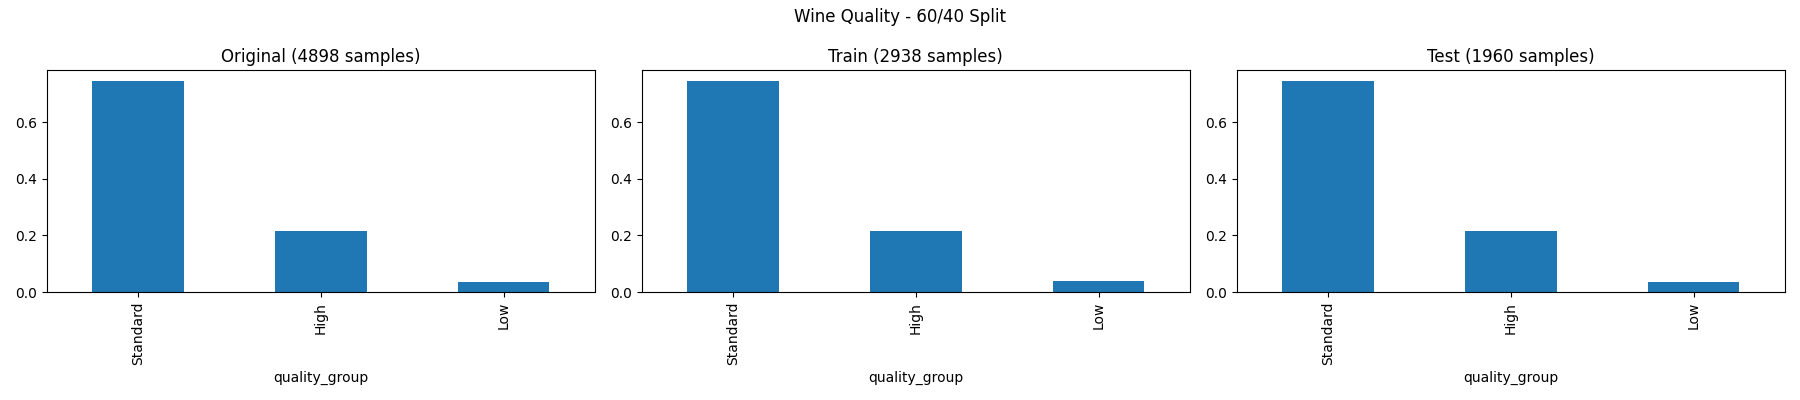
\includegraphics[width=0.6\textwidth]{imgs/class_dist/class_dist__wine_quality__60_vs_40.png}
	\caption{Wine Quality: class distribution (60/40 split).}\label{fig:wq-cd-60-40}
\end{figure}

\begin{figure}[H]
	\centering
	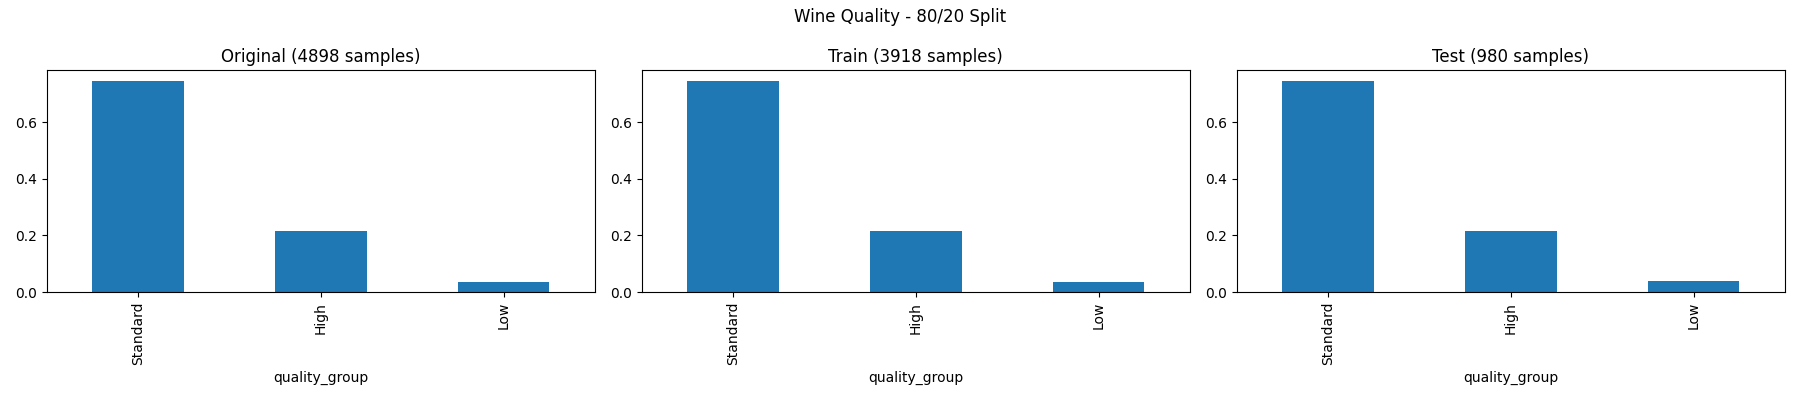
\includegraphics[width=0.6\textwidth]{imgs/class_dist/class_dist__wine_quality__80_vs_20.png}
	\caption{Wine Quality: class distribution (80/20 split).}\label{fig:wq-cd-80-20}
\end{figure}

\begin{figure}[H]
	\centering
	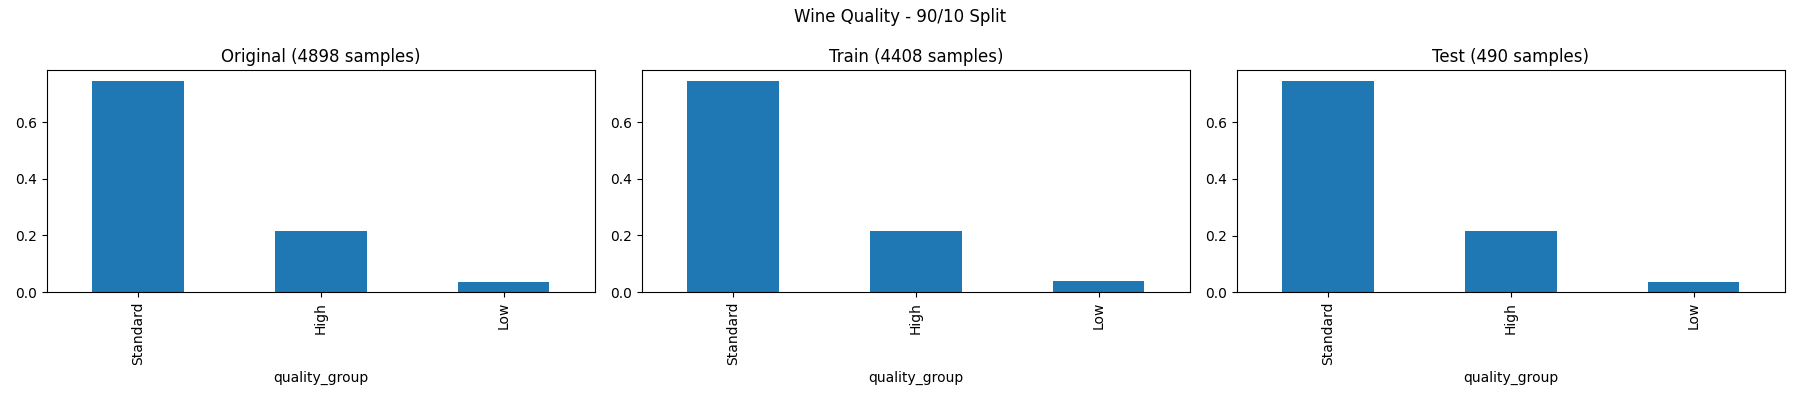
\includegraphics[width=0.6\textwidth]{imgs/class_dist/class_dist__wine_quality__90_vs_10.png}
	\caption{Wine Quality: class distribution (90/10 split).}\label{fig:wq-cd-90-10}
\end{figure}

\begin{figure}[H]
	\centering
	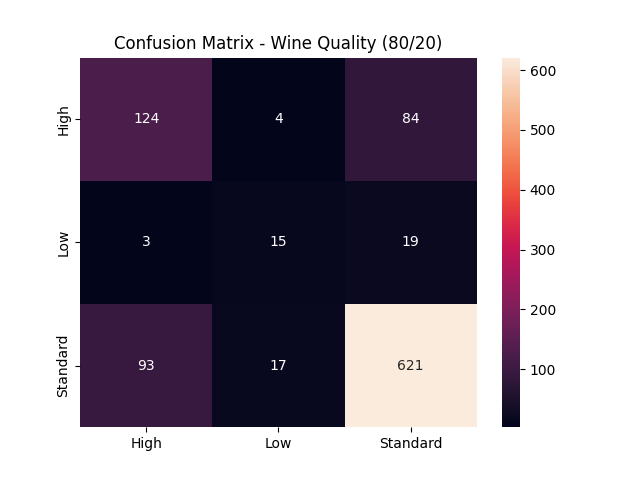
\includegraphics[width=0.6\textwidth]{imgs/confusion_mat/confusion_mat__wine_quality__80_vs_20.png}
	\caption{Wine Quality: confusion matrix (80/20 split).}\label{fig:wq-cm-80-20}
\end{figure}

% \begin{figure}[H]
% 	\centering
% 	\includegraphics[width=0.8\textwidth]{imgs/dt-mini/dt__wine_quality__80_vs_20.png}
% 	\caption{Wine Quality: decision tree (base) for 80/20 split.}\label{fig:wq-dt-base}
% \end{figure}

\begin{figure}[H]
	\centering
	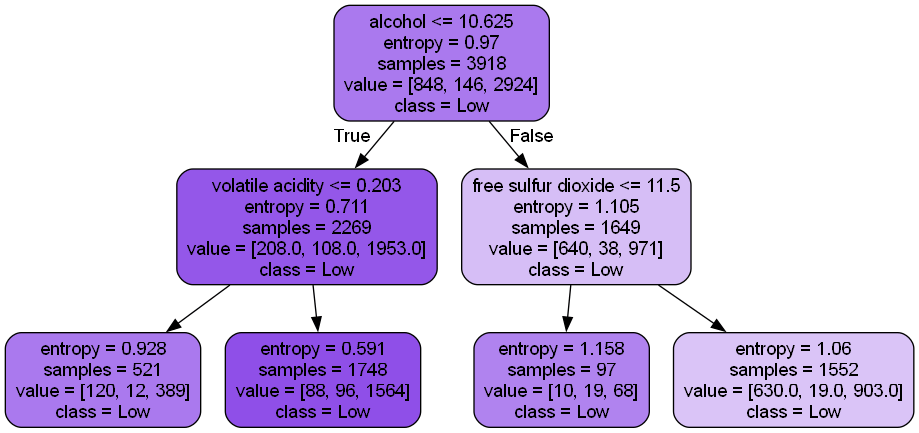
\includegraphics[width=0.8\textwidth]{imgs/dt-mini/dt__wine_quality__80_vs_20__2.png}
	\caption{Wine Quality: decision tree with \texttt{max\_depth}=2 (80/20 split).}\label{fig:wq-dt-depth-2}
\end{figure}

\begin{figure}[H]
	\centering
	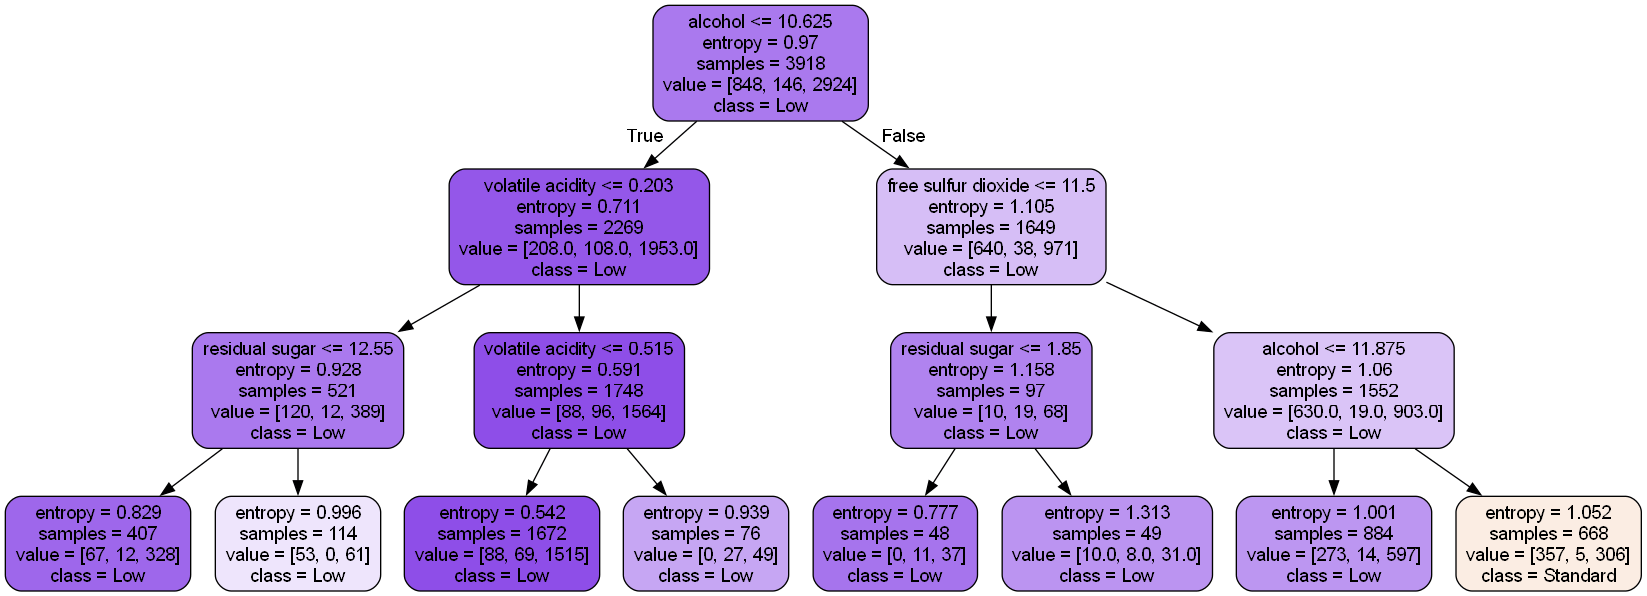
\includegraphics[width=0.8\textwidth]{imgs/dt-mini/dt__wine_quality__80_vs_20__3.png}
	\caption{Wine Quality: decision tree with \texttt{max\_depth}=3 (80/20 split).}\label{fig:wq-dt-depth-3}
\end{figure}

\begin{figure}[H]
	\centering
	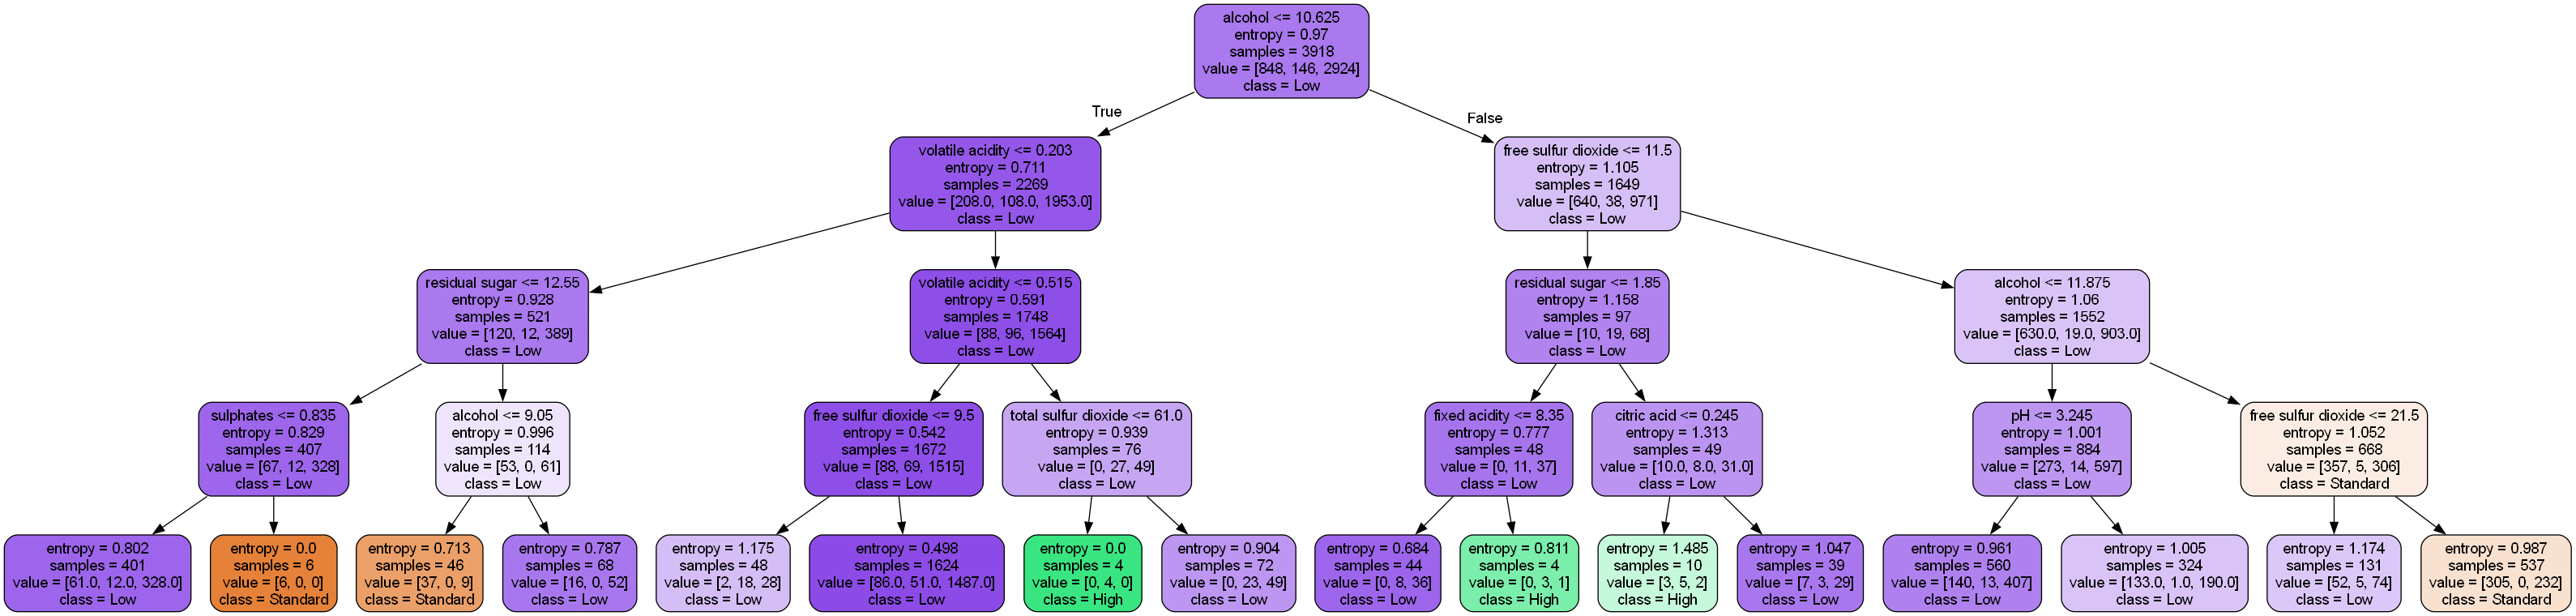
\includegraphics[width=0.8\textwidth]{imgs/dt-mini/dt__wine_quality__80_vs_20__4.png}
	\caption{Wine Quality: decision tree with \texttt{max\_depth}=4 (80/20 split).}\label{fig:wq-dt-depth-4}
\end{figure}

\begin{figure}[H]
	\centering
	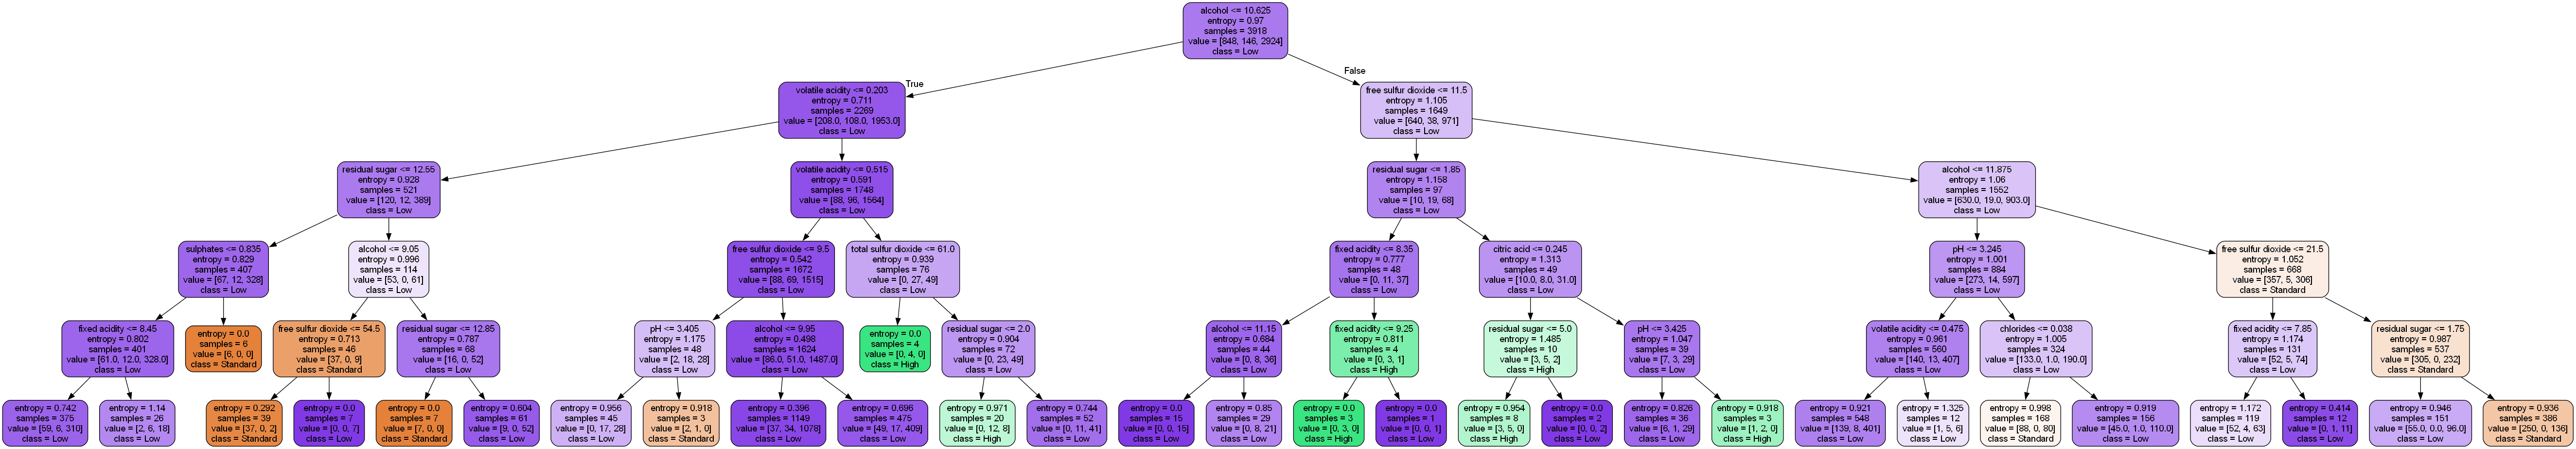
\includegraphics[width=0.8\textwidth]{imgs/dt-mini/dt__wine_quality__80_vs_20__5.png}
	\caption{Wine Quality: decision tree with \texttt{max\_depth}=5 (80/20 split).}\label{fig:wq-dt-depth-5}
\end{figure}

\begin{figure}[H]
	\centering
	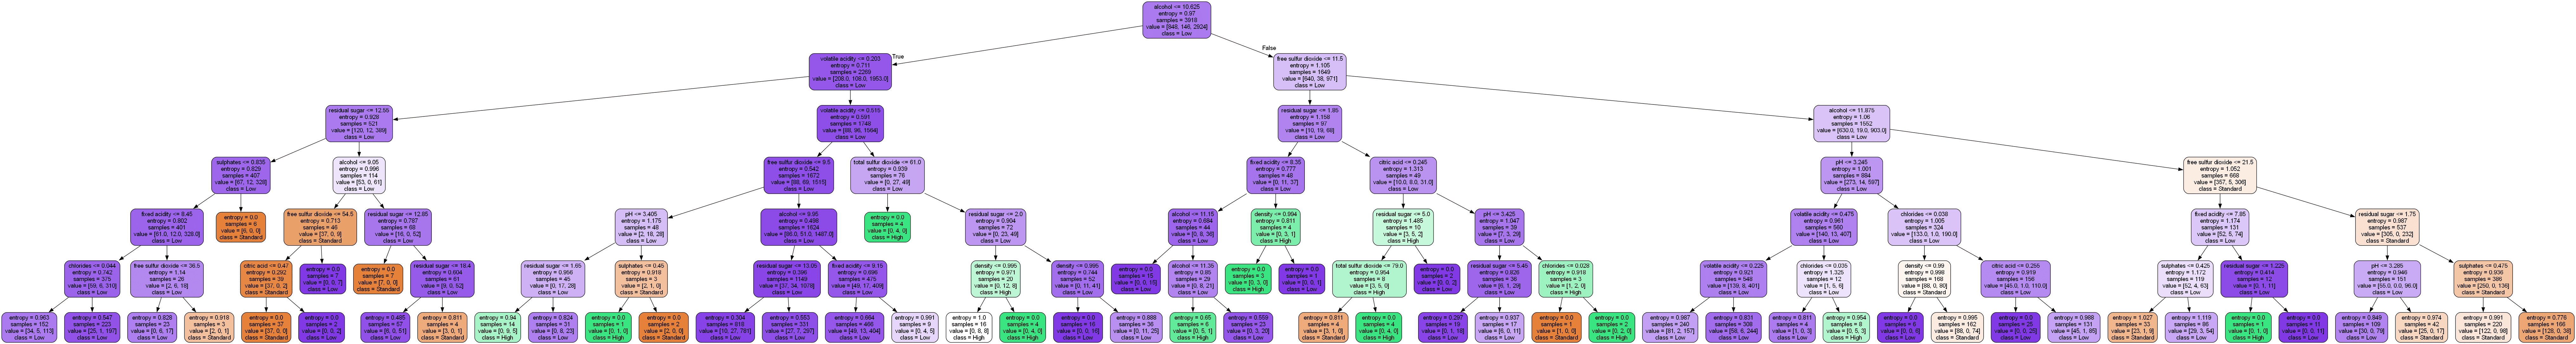
\includegraphics[width=0.8\textwidth]{imgs/dt-mini/dt__wine_quality__80_vs_20__6.png}
	\caption{Wine Quality: decision tree with \texttt{max\_depth}=6 (80/20 split).}\label{fig:wq-dt-depth-6}
\end{figure}

\begin{figure}[H]
	\centering
	
\includegraphics[width=0.8\textwidth]{imgs/dt-mini/dt__wine_quality__80_vs_20__7.png}
	\caption{Wine Quality: decision tree with \texttt{max\_depth}=7 (80/20 split).}\label{fig:wq-dt-depth-7}
\end{figure}

% \begin{figure}[H]
% 	\centering
% 	\includegraphics[width=0.8\textwidth]{imgs/dt-mini/dt__wine_quality__80_vs_20__None.png}
% 	\caption{Wine Quality: decision tree with \texttt{max\_depth}=None (80/20 split).}\label{fig:wq-dt-depth-none}
% \end{figure}

%================ Car Evaluation =================%
\clearpage
\subsection{Car Evaluation Dataset}
\begin{itemize}
	\item \textbf{Description:} 1,728 samples; 4 classes (\texttt{unacc}, \texttt{acc}, \texttt{good}, \texttt{vgood}), 6 categorical features.
	\item \textbf{Preprocessing:} label encoding, stratified splits at 40/60, 60/40, 80/20, 90/10.
\end{itemize}

\begin{figure}[H]
	\centering
	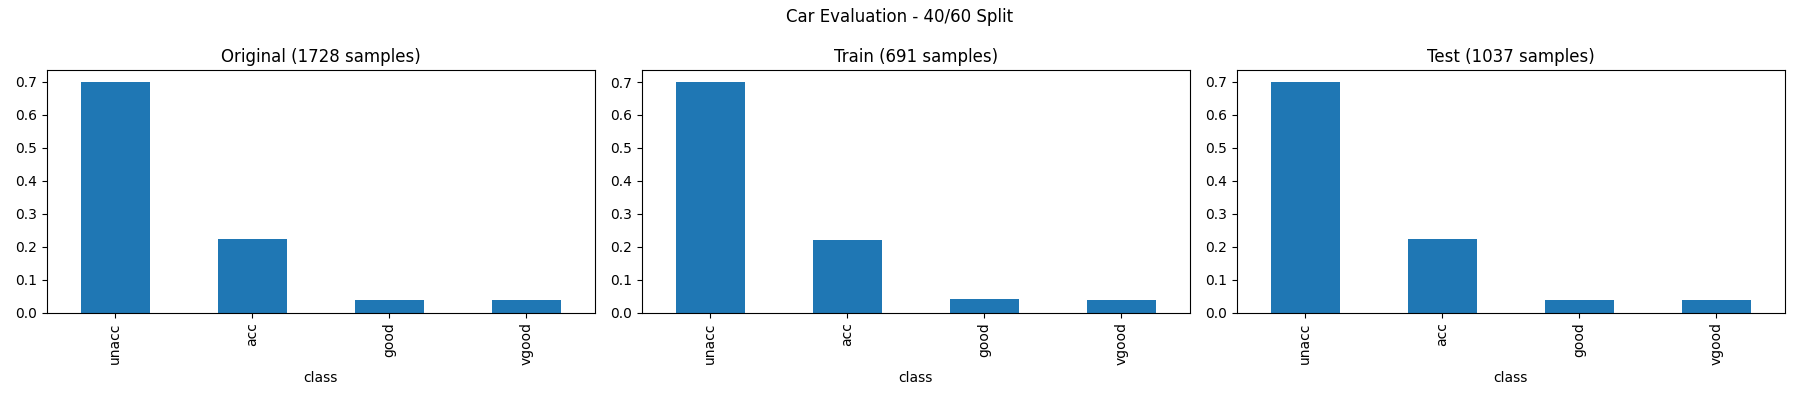
\includegraphics[width=0.6\textwidth]{imgs/class_dist/class_dist__car_evaluation__40_vs_60.png}
	\caption{Car Evaluation: class distribution (40/60 split).}\label{fig:ce-cd-40-60}
\end{figure}

\begin{figure}[H]
	\centering
	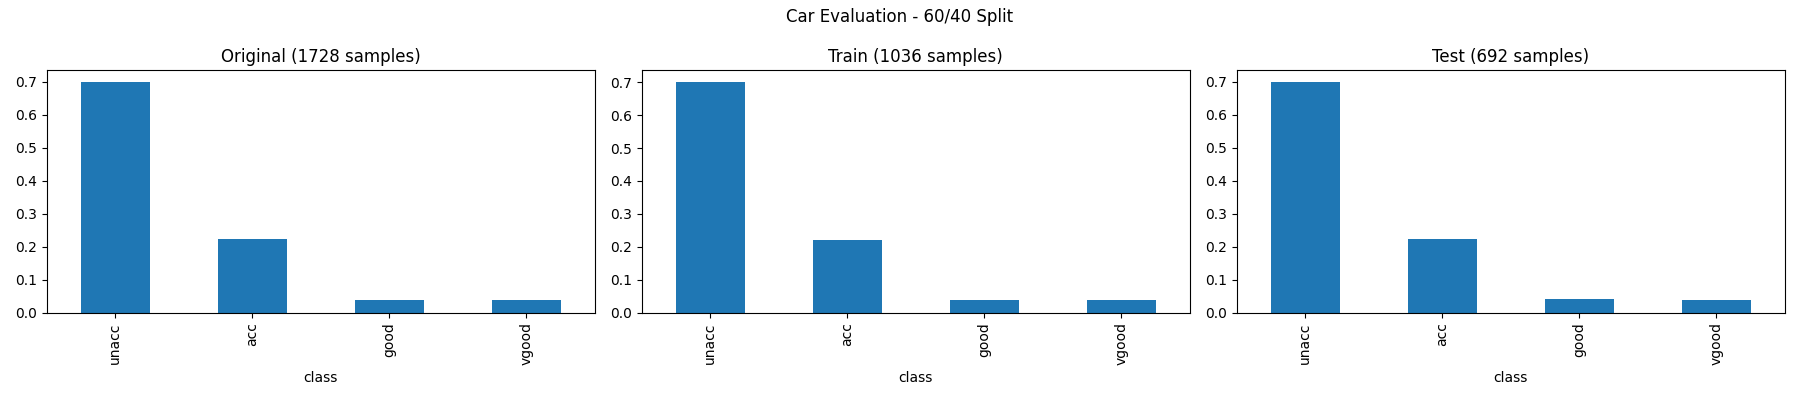
\includegraphics[width=0.6\textwidth]{imgs/class_dist/class_dist__car_evaluation__60_vs_40.png}
	\caption{Car Evaluation: class distribution (60/40 split).}\label{fig:ce-cd-60-40}
\end{figure}

\begin{figure}[H]
	\centering
	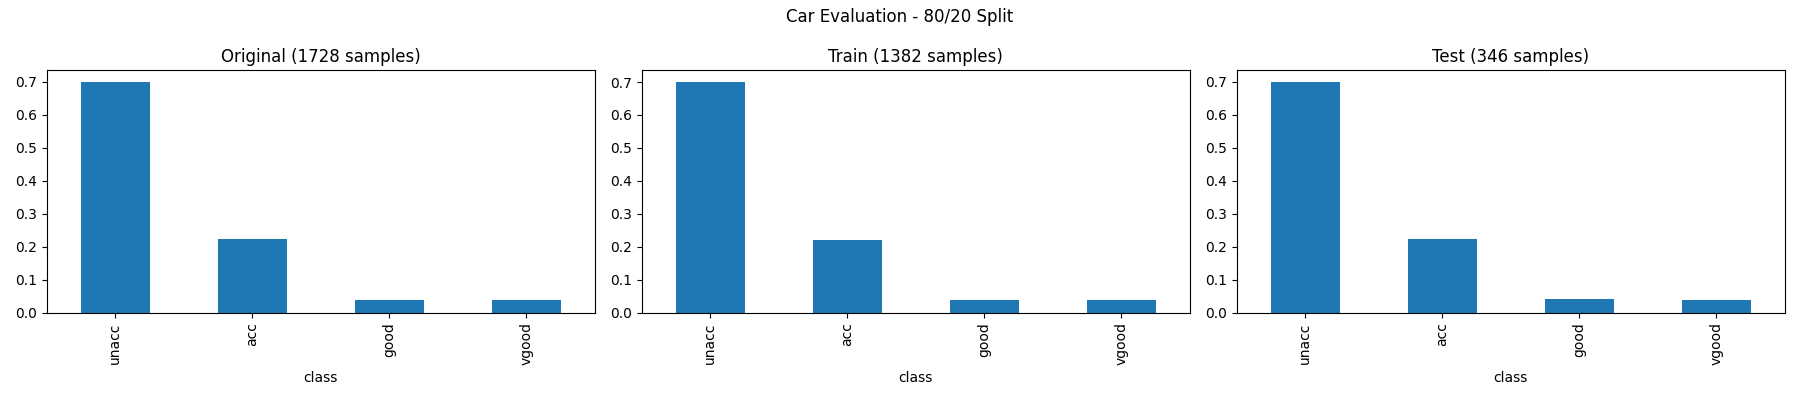
\includegraphics[width=0.6\textwidth]{imgs/class_dist/class_dist__car_evaluation__80_vs_20.png}
	\caption{Car Evaluation: class distribution (80/20 split).}\label{fig:ce-cd-80-20}
\end{figure}

\begin{figure}[H]
	\centering
	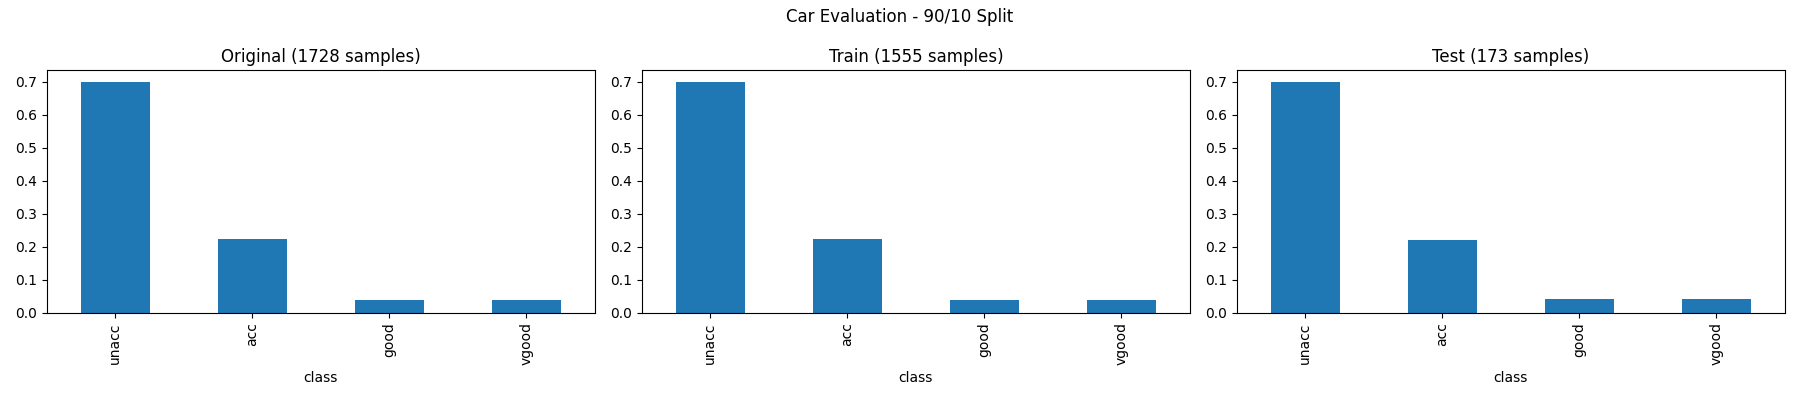
\includegraphics[width=0.6\textwidth]{imgs/class_dist/class_dist__car_evaluation__90_vs_10.png}
	\caption{Car Evaluation: class distribution (90/10 split).}\label{fig:ce-cd-90-10}
\end{figure}

\begin{figure}[H]
	\centering
	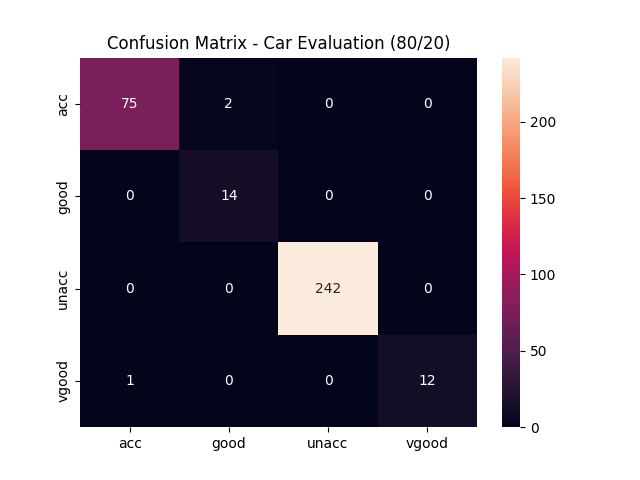
\includegraphics[width=0.6\textwidth]{imgs/confusion_mat/confusion_mat__car_evaluation__80_vs_20.png}
	\caption{Car Evaluation: confusion matrix (80/20 split).}\label{fig:ce-cm-80-20}
\end{figure}

\begin{figure}[H]
	\centering
	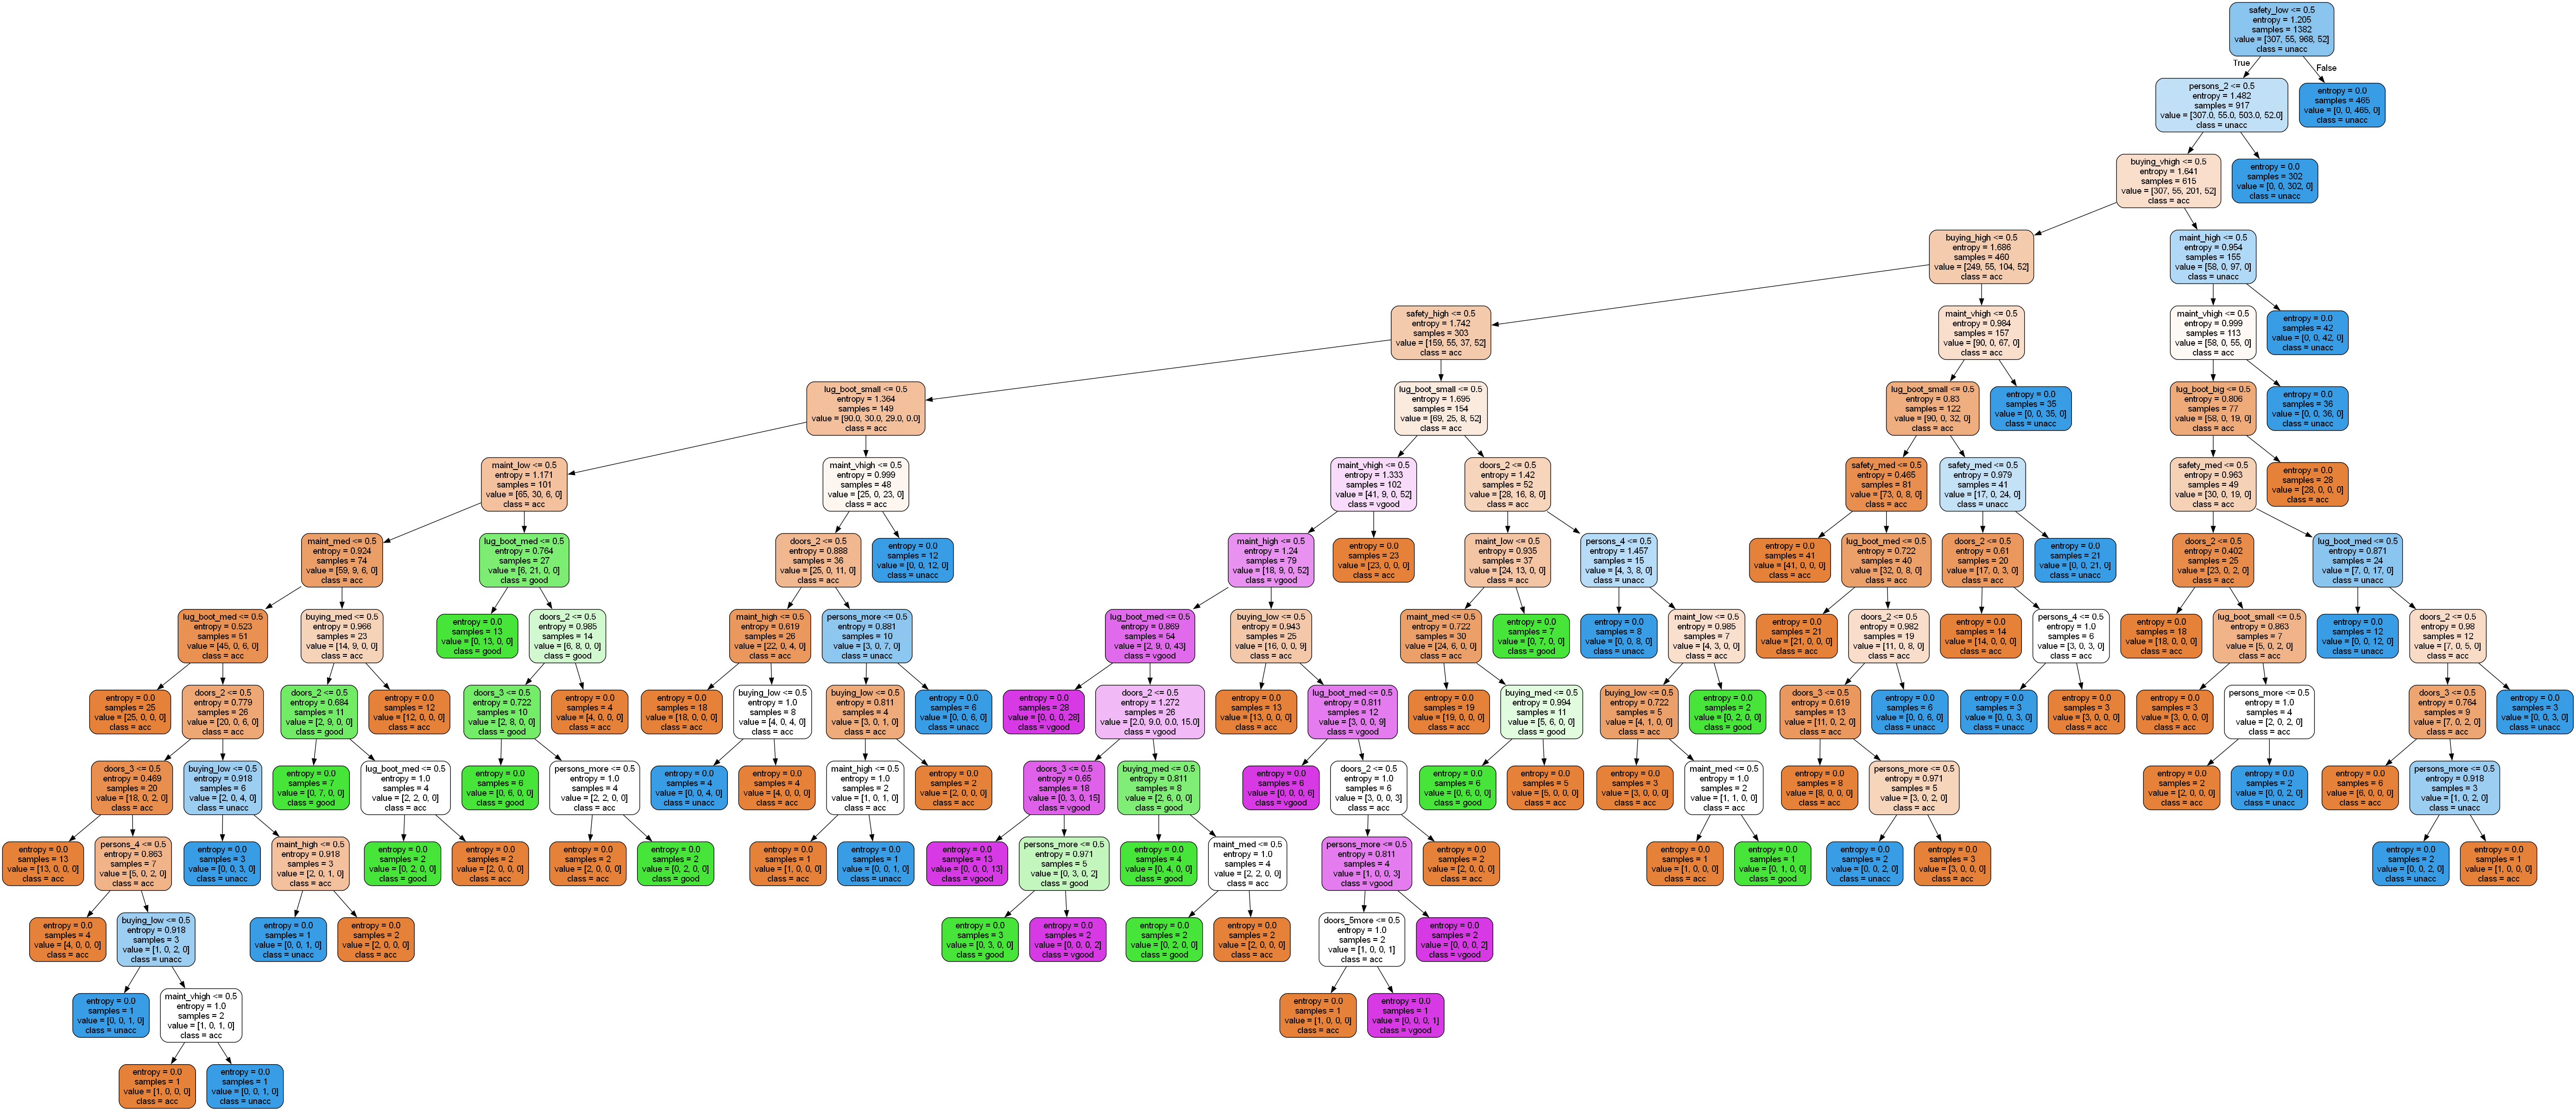
\includegraphics[width=0.8\textwidth]{imgs/dt-mini/dt__car_evaluation__80_vs_20.png}
	\caption{Car Evaluation: decision tree (base) for 80/20 split.}\label{fig:ce-dt-base}
\end{figure}

\begin{figure}[H]
	\centering
	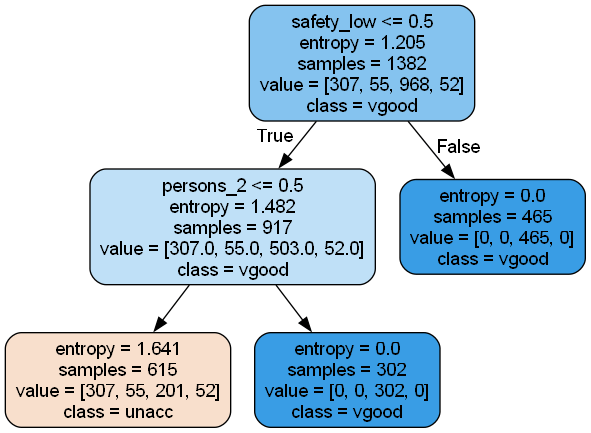
\includegraphics[width=0.8\textwidth]{imgs/dt-mini/dt__car_evaluation__80_vs_20__2.png}
	\caption{Car Evaluation: decision tree with \texttt{max\_depth}=2 (80/20 split).}\label{fig:ce-dt-depth-2}
\end{figure}

\begin{figure}[H]
	\centering
	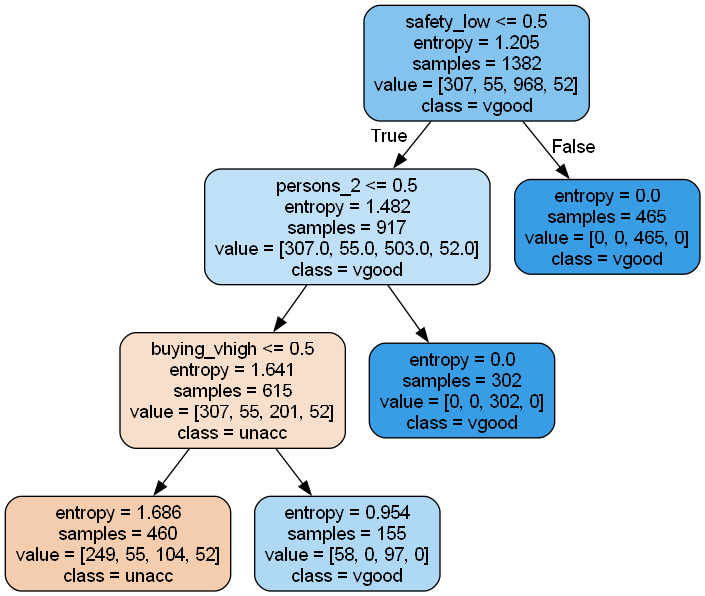
\includegraphics[width=0.8\textwidth]{imgs/dt-mini/dt__car_evaluation__80_vs_20__3.png}
	\caption{Car Evaluation: decision tree with \texttt{max\_depth}=3 (80/20 split).}\label{fig:ce-dt-depth-3}
\end{figure}

\begin{figure}[H]
	\centering
	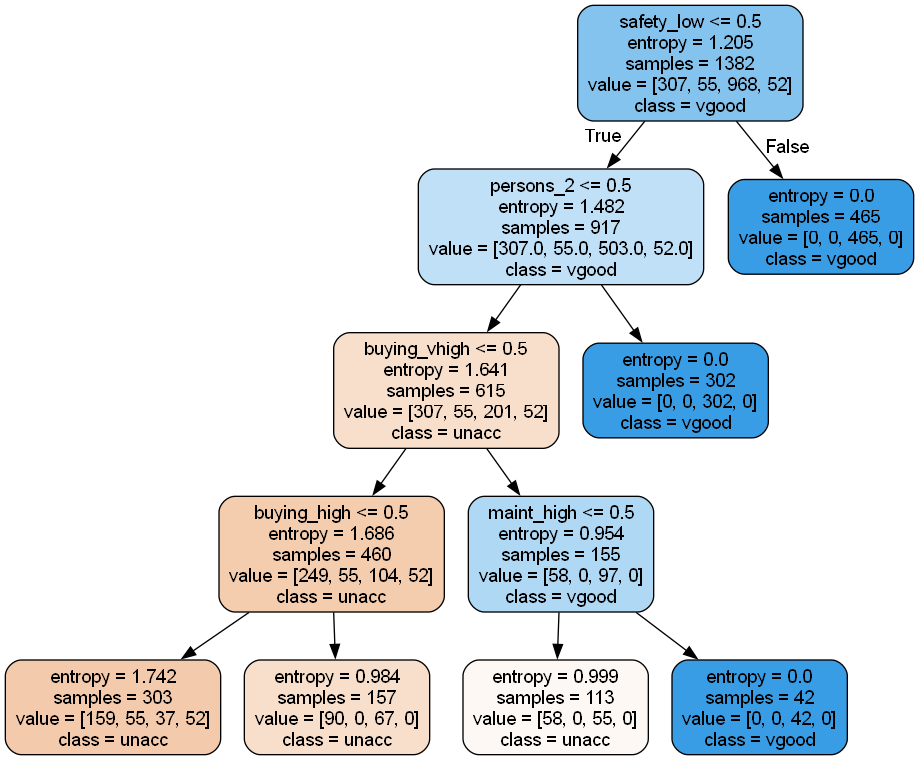
\includegraphics[width=0.8\textwidth]{imgs/dt-mini/dt__car_evaluation__80_vs_20__4.png}
	\caption{Car Evaluation: decision tree with \texttt{max\_depth}=4 (80/20 split).}\label{fig:ce-dt-depth-4}
\end{figure}

\begin{figure}[H]
	\centering
	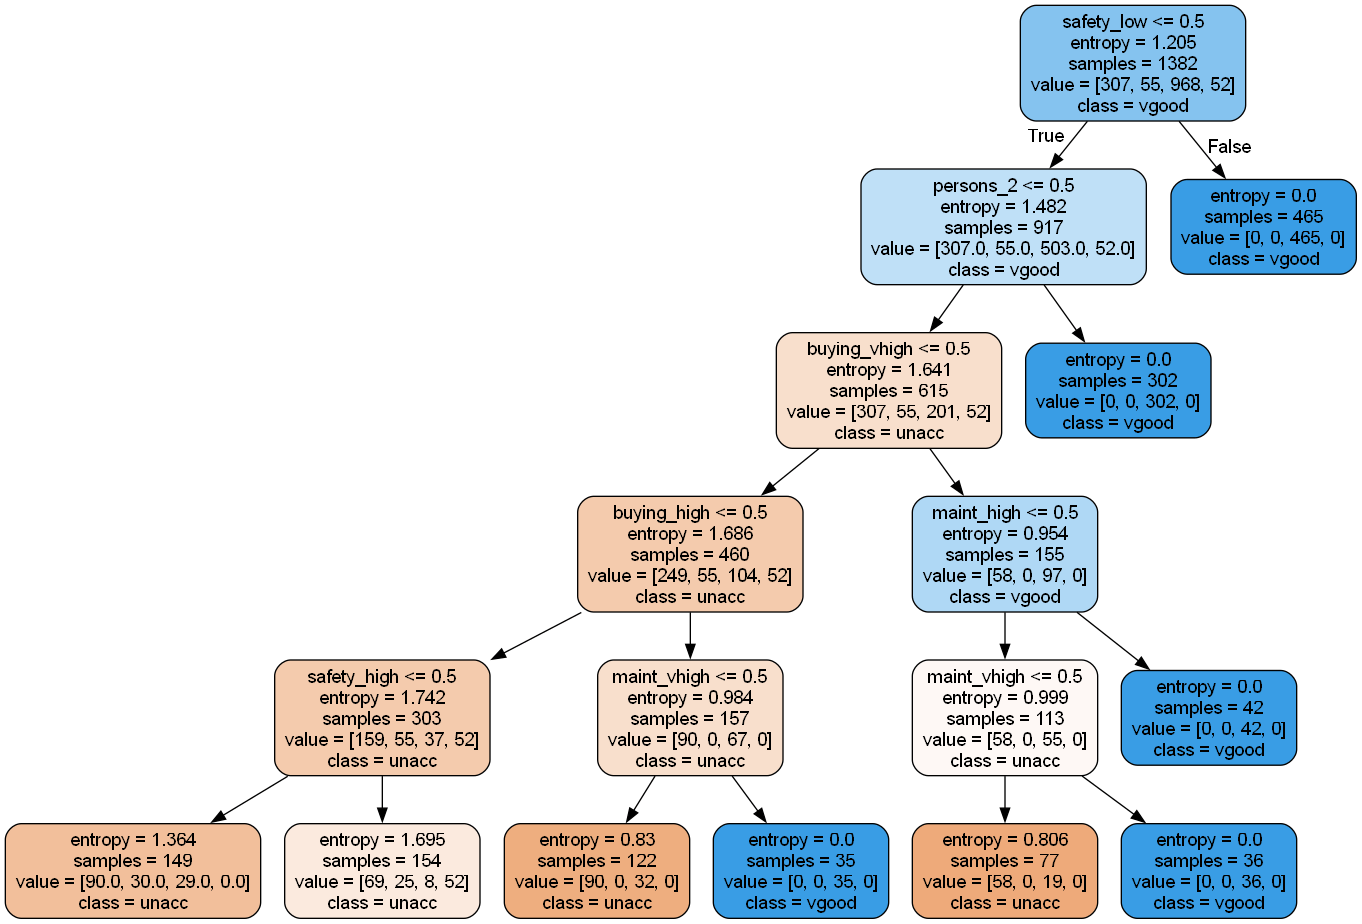
\includegraphics[width=0.8\textwidth]{imgs/dt-mini/dt__car_evaluation__80_vs_20__5.png}
	\caption{Car Evaluation: decision tree with \texttt{max\_depth}=5 (80/20 split).}\label{fig:ce-dt-depth-5}
\end{figure}

\begin{figure}[H]
	\centering
	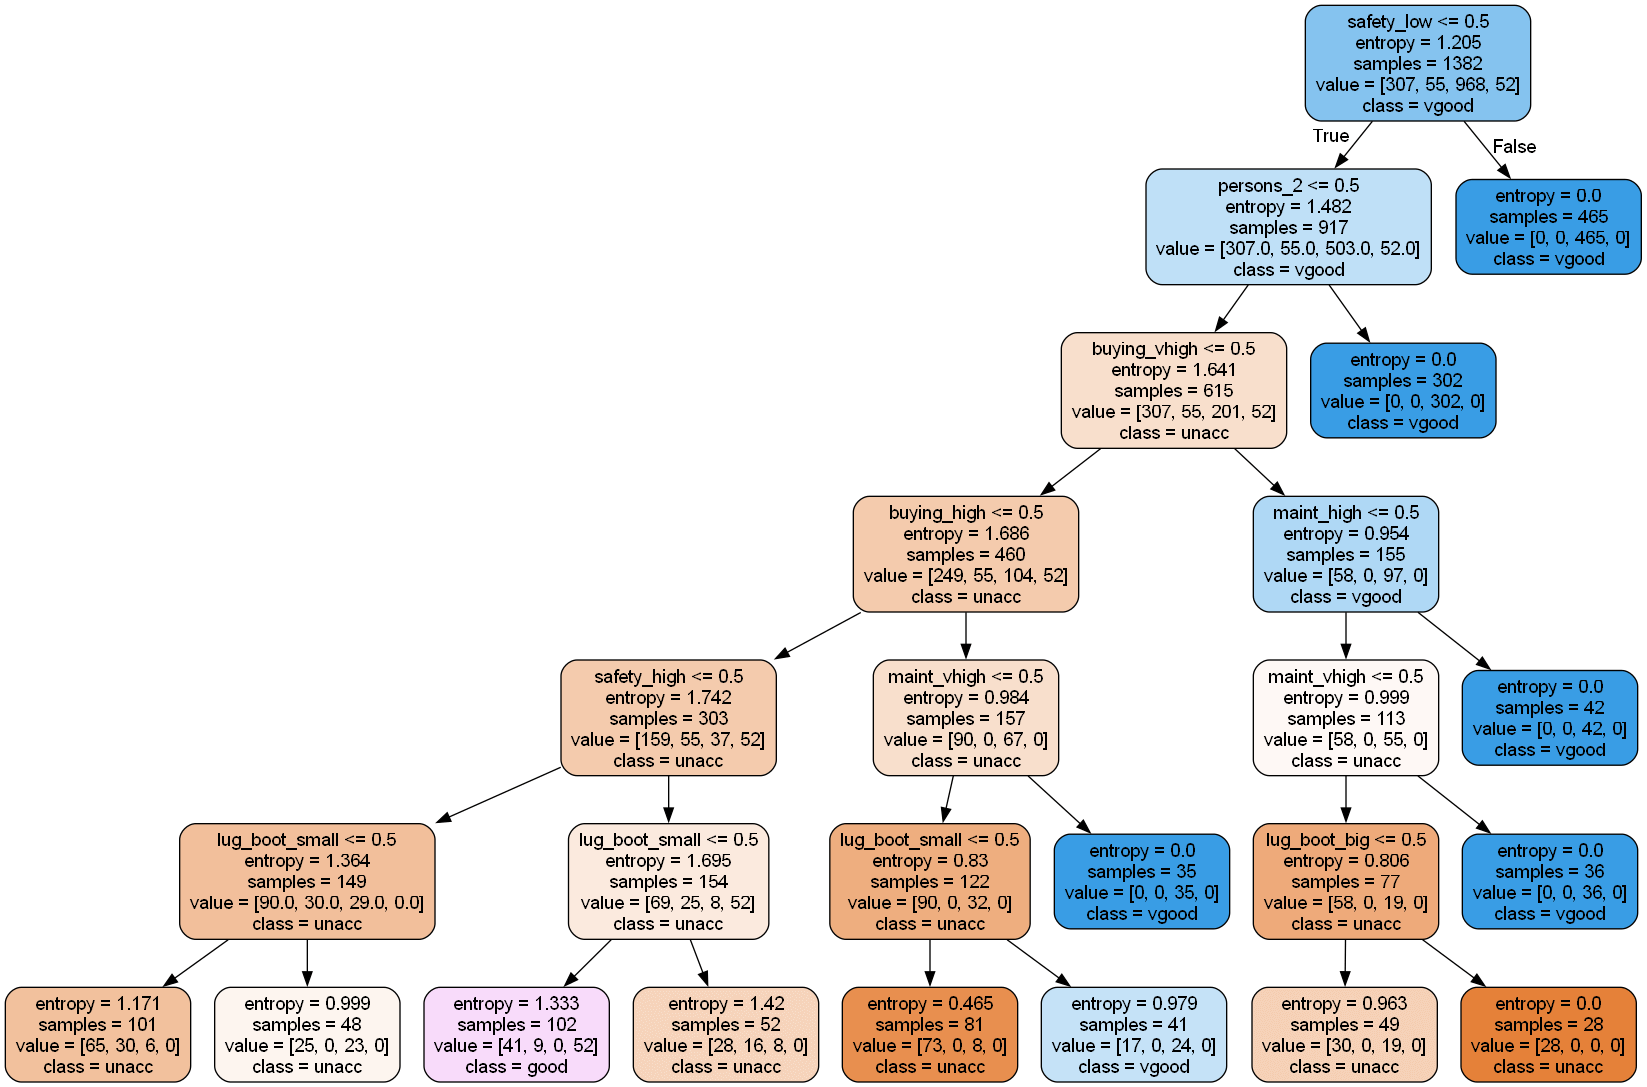
\includegraphics[width=0.8\textwidth]{imgs/dt-mini/dt__car_evaluation__80_vs_20__6.png}
	\caption{Car Evaluation: decision tree with \texttt{max\_depth}=6 (80/20 split).}\label{fig:ce-dt-depth-6}
\end{figure}

\begin{figure}[H]
	\centering
	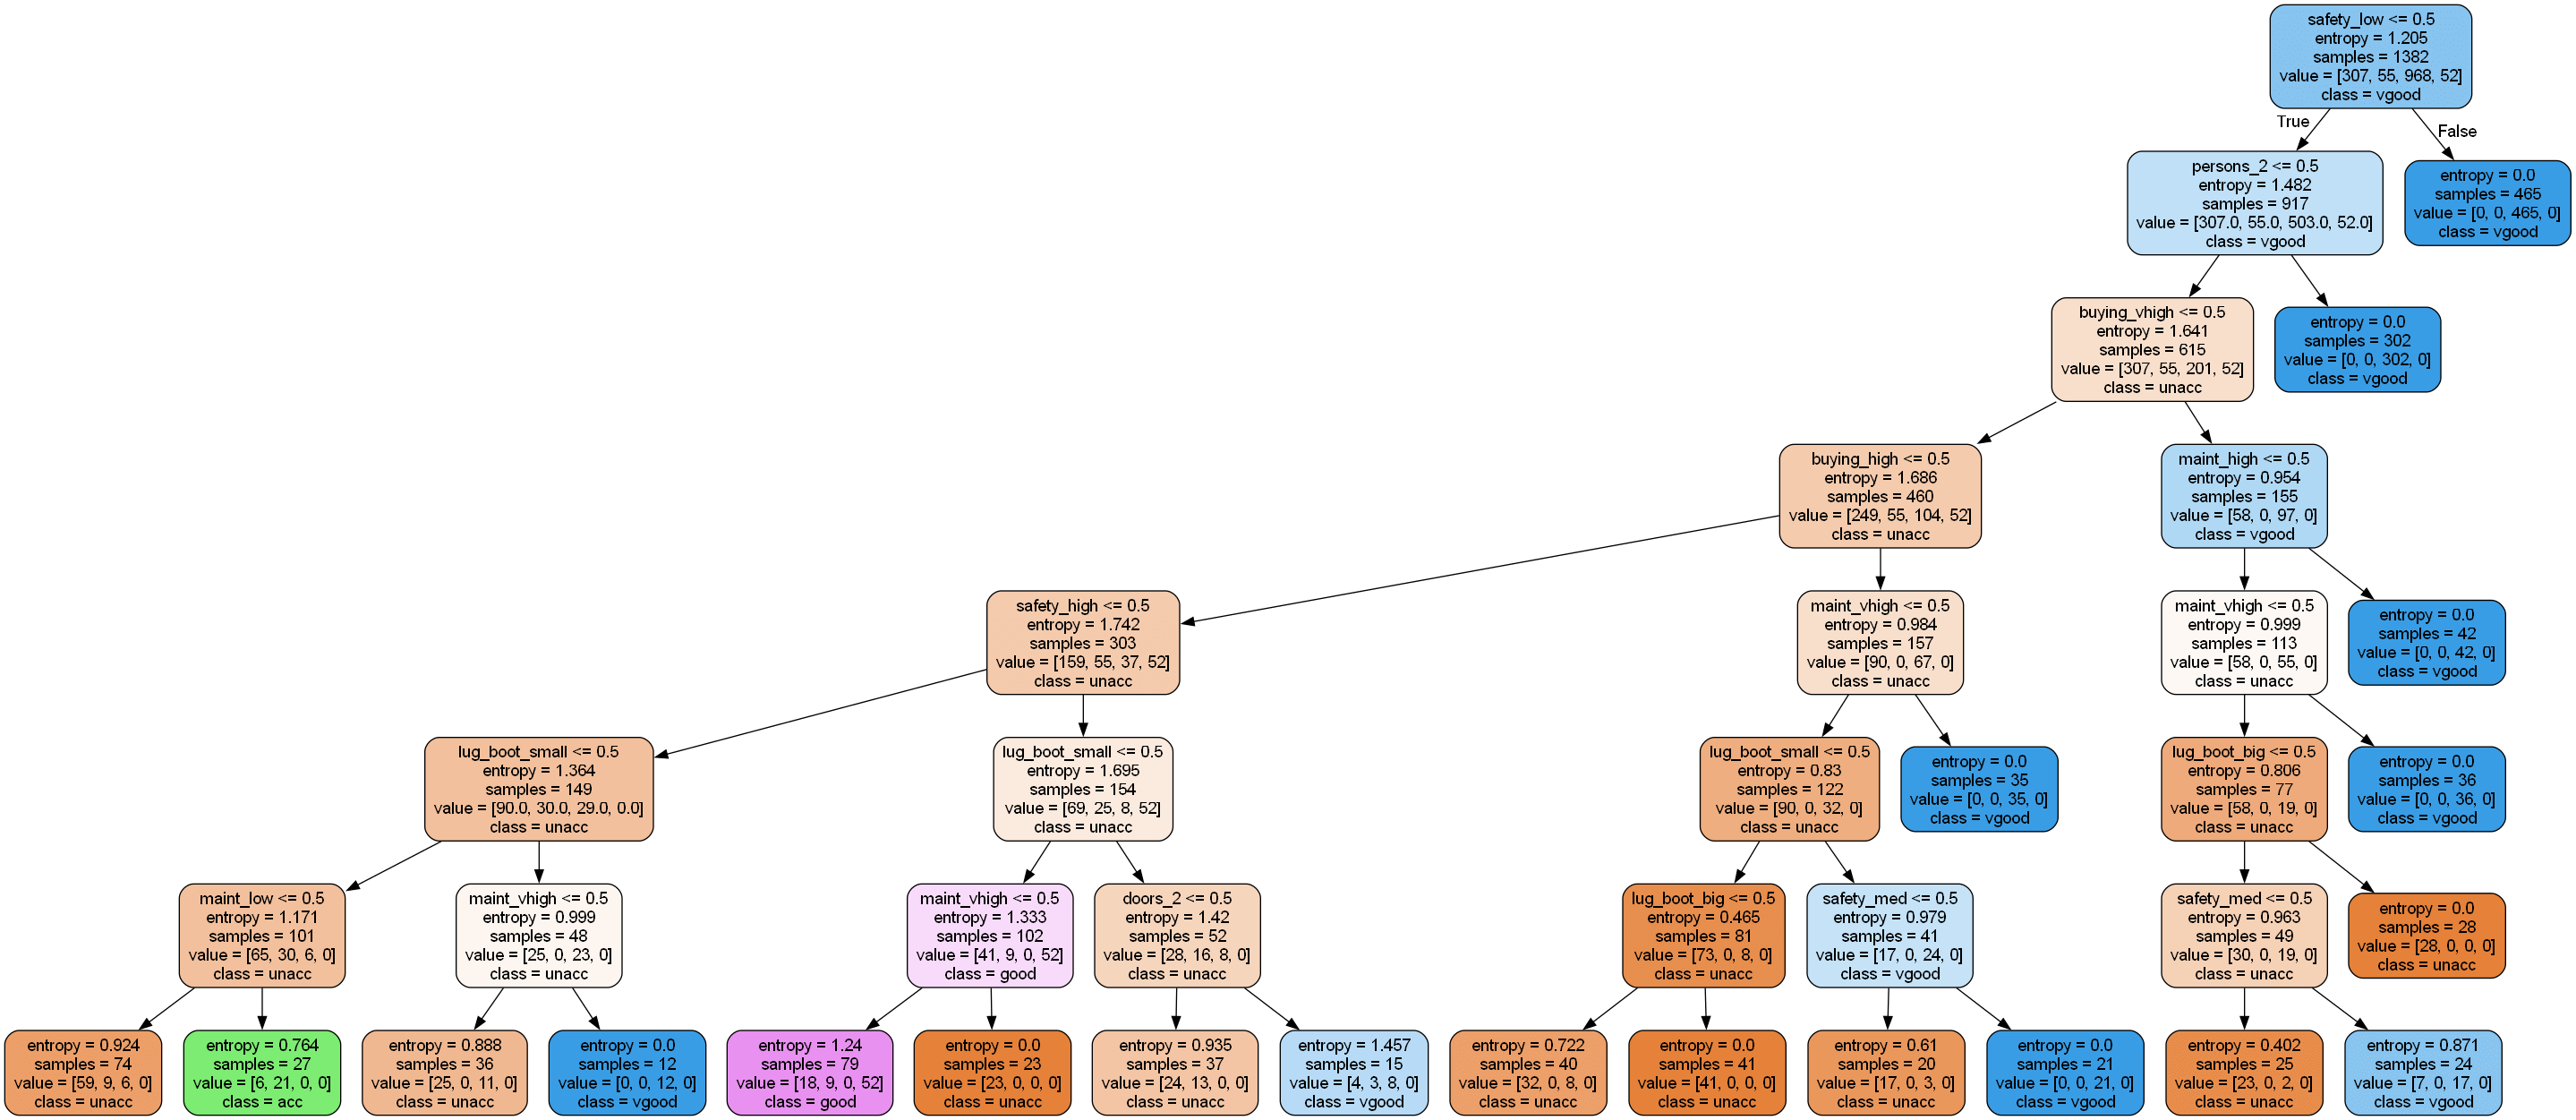
\includegraphics[width=0.8\textwidth]{imgs/dt-mini/dt__car_evaluation__80_vs_20__7.png}
	\caption{Car Evaluation: decision tree with \texttt{max\_depth}=7 (80/20 split).}\label{fig:ce-dt-depth-7}
\end{figure}

\begin{figure}[H]
	\centering
	\includegraphics[width=0.8\textwidth]{imgs/dt-mini/dt__car_evaluation__80_vs_20__None.png}
	\caption{Car Evaluation: decision tree with \texttt{max\_depth}=None (80/20 split).}\label{fig:ce-dt-depth-none}
\end{figure}
